% appendix.tex -- Supplementary material

\section{Broader Impact Statement}\label{app:broader-impact}
This work is primarily methodological: it connects two well-studied mathematical frameworks (modern Hopfield networks and Langevin dynamics) to produce a stochastic attention mechanism. Because the method generates outputs that are structured combinations of stored memory patterns, it inherits the biases present in whatever memory matrix is supplied. Practitioners should therefore audit the stored patterns for representational harms before deploying the sampler in applications that affect individuals (e.g., image synthesis, recommendation). The training-free nature of the method lowers the barrier to misuse relative to large diffusion models, but also limits expressiveness to the convex hull of the memory, reducing the risk of generating entirely novel harmful content. We do not foresee direct negative societal consequences beyond those common to all generative modeling research, and we encourage responsible use.

\section{Proof of Proposition~\ref{prop:regularity}}\label{app:proof-regularity}

We prove the two regularity properties of the modern Hopfield energy $E$ defined in~\eqref{eq:modern-hopfield-energy}. Write $\mathbf{p}(\boldsymbol{\xi})=\operatorname{softmax}(\beta\mathbf{X}^{\top}\boldsymbol{\xi})\in\mathbb{R}^K$ for the attention weight vector at state $\boldsymbol{\xi}$, and recall the retrieval map $\mathbf{T}(\boldsymbol{\xi})=\mathbf{X}\mathbf{p}(\boldsymbol{\xi})$.

\paragraph{Hessian computation.}
The gradient is $\nabla E(\boldsymbol{\xi})=\boldsymbol{\xi}-\mathbf{T}(\boldsymbol{\xi})$~\cite{ramsauerHopfieldNetworksAll2021}. To obtain the Hessian we differentiate the retrieval map. Let $\mathbf{z}=\beta\mathbf{X}^{\top}\boldsymbol{\xi}\in\mathbb{R}^K$ denote the pre-softmax logits. The Jacobian of the softmax is the $K\times K$ matrix
\begin{equation}\label{eq:softmax-jacobian}
    \frac{\partial\mathbf{p}}{\partial\mathbf{z}}
    = \operatorname{diag}(\mathbf{p}) - \mathbf{p}\mathbf{p}^{\top}
    =: \mathbf{S}(\mathbf{p}),
\end{equation}
which is the covariance matrix of a categorical distribution with probabilities~$\mathbf{p}$. By the chain rule ($\partial\mathbf{z}/\partial\boldsymbol{\xi}=\beta\mathbf{X}^{\top}$):
\begin{equation}\label{eq:hessian}
    \nabla^{2}E(\boldsymbol{\xi})
    = \mathbf{I}_{d} - \beta\,\mathbf{X}\,\mathbf{S}\bigl(\mathbf{p}(\boldsymbol{\xi})\bigr)\,\mathbf{X}^{\top}.
\end{equation}

\paragraph{Part (i): Lipschitz gradient.}
The Lipschitz constant of $\nabla E$ equals $\sup_{\boldsymbol{\xi}}\|\nabla^{2}E(\boldsymbol{\xi})\|_{\mathrm{op}}$. Because $\mathbf{S}(\mathbf{p})$ is a covariance matrix it is positive semidefinite, so $\beta\mathbf{X}\mathbf{S}\mathbf{X}^{\top}\succeq\mathbf{0}$. By the triangle inequality for the spectral norm,
\begin{equation}\label{eq:lip-triangle}
    \|\nabla^{2}E(\boldsymbol{\xi})\|_{\mathrm{op}}
    \;\le\; \|\mathbf{I}_{d}\|_{\mathrm{op}}
            + \beta\,\|\mathbf{X}\,\mathbf{S}(\mathbf{p})\,\mathbf{X}^{\top}\|_{\mathrm{op}}
    \;\le\; 1 + \beta\,\sigma_{\max}^{2}\,\|\mathbf{S}(\mathbf{p})\|_{\mathrm{op}},
\end{equation}
where the second step uses submultiplicativity of the spectral norm: $\|\mathbf{A}\mathbf{B}\mathbf{C}\|_{\mathrm{op}}\le\|\mathbf{A}\|_{\mathrm{op}}\|\mathbf{B}\|_{\mathrm{op}}\|\mathbf{C}\|_{\mathrm{op}}$.

It remains to bound $\|\mathbf{S}(\mathbf{p})\|_{\mathrm{op}}$. For any unit vector $\mathbf{v}\in\mathbb{R}^K$,
\begin{align*}
\mathbf{v}^{\top}\mathbf{S}(\mathbf{p})\mathbf{v}
= \sum_{i}p_{i}v_{i}^{2} - \Bigl(\sum_{i}p_{i}v_{i}\Bigr)^{\!2}
= \operatorname{Var}_{\mathbf{p}}(V),
\end{align*}
where $V$ is the random variable taking value $v_i$ with probability $p_i$. By Popoviciu's variance inequality, $\operatorname{Var}(V)\le(v_{\max}-v_{\min})^{2}/4$. Under the constraint $\|\mathbf{v}\|_{2}=1$, the difference $v_{\max}-v_{\min}$ satisfies
\begin{align*}
(v_{\max}-v_{\min})^{2}
\;\le\; (|v_{\max}|+|v_{\min}|)^{2}
\;\le\; 2(v_{\max}^{2}+v_{\min}^{2})
\;\le\; 2\|\mathbf{v}\|_{2}^{2} = 2,
\end{align*}
where the second step is the Cauchy--Schwarz (QM-AM) inequality $(a+b)^{2}\le 2(a^{2}+b^{2})$ for $a,b\ge 0$. Therefore
\begin{equation}\label{eq:softmax-spectral-bound}
    \|\mathbf{S}(\mathbf{p})\|_{\mathrm{op}}
    = \sup_{\|\mathbf{v}\|=1}\operatorname{Var}_{\mathbf{p}}(V)
    \;\le\; \frac{2}{4} = \frac{1}{2},
\end{equation}
and this bound is tight: equality holds when $K\ge 2$ with $\mathbf{p}=(\tfrac{1}{2},\tfrac{1}{2},0,\dots,0)$ and $\mathbf{v}=(\tfrac{1}{\sqrt{2}},-\tfrac{1}{\sqrt{2}},0,\dots,0)$.

Substituting~\eqref{eq:softmax-spectral-bound} into~\eqref{eq:lip-triangle} yields
\begin{align*}
\sup_{\boldsymbol{\xi}}\|\nabla^{2}E(\boldsymbol{\xi})\|_{\mathrm{op}}
\;\le\; 1 + \frac{\beta\,\sigma_{\max}^{2}}{2}
=: L.
\end{align*}

\paragraph{Part (ii): Dissipativity.}
Expanding the inner product,
\begin{align*}
\langle\nabla E(\boldsymbol{\xi}),\,\boldsymbol{\xi}\rangle
= \|\boldsymbol{\xi}\|_{2}^{2} - \langle\mathbf{T}(\boldsymbol{\xi}),\,\boldsymbol{\xi}\rangle.
\end{align*}
The retrieval map $\mathbf{T}(\boldsymbol{\xi})=\mathbf{X}\mathbf{p}=\sum_{k}p_{k}\mathbf{m}_{k}$ is a convex combination of stored patterns, so by the triangle inequality
\begin{align*}
\|\mathbf{T}(\boldsymbol{\xi})\|_{2}
= \Bigl\|\sum_{k}p_{k}\mathbf{m}_{k}\Bigr\|_{2}
\le \sum_{k}p_{k}\|\mathbf{m}_{k}\|_{2}
\le M,
\end{align*}
where $M=\max_{k}\|\mathbf{m}_{k}\|_{2}$ and $\sum_{k}p_{k}=1$. By the Cauchy--Schwarz inequality,
\begin{align*}
|\langle\mathbf{T}(\boldsymbol{\xi}),\,\boldsymbol{\xi}\rangle|
\le \|\mathbf{T}(\boldsymbol{\xi})\|_{2}\,\|\boldsymbol{\xi}\|_{2}
\le M\|\boldsymbol{\xi}\|_{2}.
\end{align*}
Applying Young's inequality $ab\le\tfrac{a^{2}}{2}+\tfrac{b^{2}}{2}$ with $a=M$ and $b=\|\boldsymbol{\xi}\|_{2}$,
\begin{align*}
M\|\boldsymbol{\xi}\|_{2}
\;\le\; \frac{M^{2}}{2} + \frac{\|\boldsymbol{\xi}\|_{2}^{2}}{2}.
\end{align*}
Hence
\begin{align*}
\langle\nabla E(\boldsymbol{\xi}),\,\boldsymbol{\xi}\rangle
\;\ge\; \|\boldsymbol{\xi}\|_{2}^{2} - \frac{M^{2}}{2} - \frac{\|\boldsymbol{\xi}\|_{2}^{2}}{2}
= \frac{1}{2}\|\boldsymbol{\xi}\|_{2}^{2} - \frac{M^{2}}{2},
\end{align*}
which is the dissipativity condition \textbf{(R2)} with constants $a=\tfrac{1}{2}$ and $b=\tfrac{M^{2}}{2}$. \qed

\paragraph{Convexity threshold (Corollary~\ref{cor:convergence}).}
Since $\mathbf{S}(\mathbf{p})\succeq\mathbf{0}$, the Hessian~\eqref{eq:hessian} satisfies $\nabla^{2}E\preceq\mathbf{I}$ (the identity provides an upper bound on the eigenvalues). For the lower bound, $\beta\mathbf{X}\mathbf{S}\mathbf{X}^{\top}\preceq\tfrac{\beta\sigma_{\max}^{2}}{2}\mathbf{I}$ by~\eqref{eq:softmax-spectral-bound} and submultiplicativity, so
\begin{align*}
\nabla^{2}E(\boldsymbol{\xi})
\;\succeq\; \Bigl(1-\frac{\beta\sigma_{\max}^{2}}{2}\Bigr)\mathbf{I}.
\end{align*}
When $\beta\sigma_{\max}^{2}<2$ the lower bound is strictly positive, so $E$ is strictly convex. The potential $U=\beta E$ is then $m$-strongly convex with $m=\beta(1-\beta\sigma_{\max}^{2}/2)$ and has $L_{U}$-Lipschitz gradient with $L_{U}=\beta(1+\beta\sigma_{\max}^{2}/2)$. The condition number is
\begin{align*}
\kappa = \frac{L_{U}}{m}
= \frac{1+\beta\sigma_{\max}^{2}/2}{1-\beta\sigma_{\max}^{2}/2},
\end{align*}
which diverges as $\beta\sigma_{\max}^{2}\to 2$, reflecting the onset of non-convexity and the proliferation of local minima in the energy landscape.


\section{MALA Variant of Stochastic Attention}\label{app:mala-algorithm}

Algorithm~\ref{alg:stochastic-attention} uses the Unadjusted Langevin Algorithm (ULA), which is simple but introduces an $O(\alpha)$ discretization bias. The Metropolis-Adjusted Langevin Algorithm (MALA) eliminates this bias by appending an accept/reject step to each Langevin proposal. At the step size and temperature used in our experiments ($\alpha{=}0.01$, $\beta{=}2000$), the two algorithms produced practically indistinguishable outputs (Table~\ref{tab:mnist-baselines}); however, the correction becomes important when a larger step size is desired, e.g., to accelerate mixing in high-dimensional or low-temperature settings where $\alpha$ must be increased beyond the regime in which the ULA bias is negligible.

\begin{algorithm}[h]
\caption{MALA Stochastic Attention Sampler}\label{alg:mala}
\begin{algorithmic}[1]
\REQUIRE Memory matrix $\mathbf{X}\in\mathbb{R}^{d\times K}$, inverse temperature $\beta>0$, step size $\alpha\in(0,1)$, iterations $T$, initial state $\boldsymbol{\xi}_0\in\mathbb{R}^d$
\ENSURE Sample trajectory $\boldsymbol{\xi}_0,\boldsymbol{\xi}_1,\dots,\boldsymbol{\xi}_T$
\FOR{$t = 0,1,\dots,T-1$}
    \STATE $\mathbf{a}_t \leftarrow \operatorname{softmax}\!\bigl(\beta\,\mathbf{X}^{\top}\boldsymbol{\xi}_t\bigr)$ \hfill $\triangleright$ attention weights at current state
    \STATE $\boldsymbol{\mu}_t \leftarrow (1-\alpha)\,\boldsymbol{\xi}_t + \alpha\,\mathbf{X}\,\mathbf{a}_t$ \hfill $\triangleright$ Langevin proposal mean
    \STATE $\boldsymbol{\epsilon}_t \sim \mathcal{N}(\mathbf{0},\mathbf{I}_d)$
    \STATE $\boldsymbol{\xi}^{\star} \leftarrow \boldsymbol{\mu}_t + \sqrt{2\alpha/\beta}\;\boldsymbol{\epsilon}_t$ \hfill $\triangleright$ candidate state
    \STATE $\mathbf{a}^{\star} \leftarrow \operatorname{softmax}\!\bigl(\beta\,\mathbf{X}^{\top}\boldsymbol{\xi}^{\star}\bigr)$ \hfill $\triangleright$ attention weights at candidate
    \STATE $\boldsymbol{\mu}^{\star} \leftarrow (1-\alpha)\,\boldsymbol{\xi}^{\star} + \alpha\,\mathbf{X}\,\mathbf{a}^{\star}$ \hfill $\triangleright$ reverse proposal mean
    \STATE $\log r \leftarrow -\beta\bigl[E(\boldsymbol{\xi}^{\star}) - E(\boldsymbol{\xi}_t)\bigr]
             - \frac{\beta}{4\alpha}\bigl[\lVert\boldsymbol{\xi}_t - \boldsymbol{\mu}^{\star}\rVert^2
             - \lVert\boldsymbol{\xi}^{\star} - \boldsymbol{\mu}_t\rVert^2\bigr]$
    \STATE $u \sim \mathrm{Uniform}(0,1)$
    \IF{$\log u < \min(0,\,\log r)$}
        \STATE $\boldsymbol{\xi}_{t+1} \leftarrow \boldsymbol{\xi}^{\star}$ \hfill $\triangleright$ accept
    \ELSE
        \STATE $\boldsymbol{\xi}_{t+1} \leftarrow \boldsymbol{\xi}_t$ \hfill $\triangleright$ reject
    \ENDIF
\ENDFOR
\end{algorithmic}
\end{algorithm}

Compared with Algorithm~\ref{alg:stochastic-attention}, MALA replaces the single-line state update (line~4) with a propose-then-correct cycle (lines~2--13). The additional cost per step is one extra attention evaluation (line~6) and one energy evaluation (line~8), doubling the per-iteration $\mathcal{O}(dK)$ cost. In the limit $\alpha\to 0$ both algorithms coincide; at moderate $\alpha$ the accept/reject step removes $O(\alpha)$ discretization bias.

\paragraph{What line~8 computes and why.}
The ULA update in Algorithm~\ref{alg:stochastic-attention} draws each new state from a Gaussian proposal centered on the Langevin mean $\boldsymbol{\mu}_t$:
\begin{equation}\label{eq:mala-forward}
q(\boldsymbol{\xi}^{\star}\mid\boldsymbol{\xi}_t)
= \mathcal{N}\!\bigl(\boldsymbol{\xi}^{\star};\;\boldsymbol{\mu}_t,\;\tfrac{2\alpha}{\beta}\mathbf{I}\bigr),
\end{equation}
where $\boldsymbol{\mu}_t = (1{-}\alpha)\boldsymbol{\xi}_t + \alpha\,\mathbf{X}\mathbf{a}_t$ encodes one step of gradient descent on $E$.
For the chain to sample from the correct Boltzmann target $p_\beta\propto\exp(-\beta E)$, the transition kernel must satisfy \emph{detailed balance}: $p_\beta(\boldsymbol{\xi})\,q(\boldsymbol{\xi}^{\star}\mid\boldsymbol{\xi}) = p_\beta(\boldsymbol{\xi}^{\star})\,q(\boldsymbol{\xi}\mid\boldsymbol{\xi}^{\star})$ for every pair of states.
When $\alpha>0$ the proposal~\eqref{eq:mala-forward} is \emph{asymmetric}: the forward density $q(\boldsymbol{\xi}^{\star}\mid\boldsymbol{\xi}_t)$ is centered on $\boldsymbol{\mu}_t$, but the reverse density $q(\boldsymbol{\xi}_t\mid\boldsymbol{\xi}^{\star})$ is centered on a \emph{different} point $\boldsymbol{\mu}^{\star}=(1{-}\alpha)\boldsymbol{\xi}^{\star}+\alpha\mathbf{X}\mathbf{a}^{\star}$ (line~7). The gradient at the candidate $\boldsymbol{\xi}^{\star}$ generally differs from the gradient at $\boldsymbol{\xi}_t$, so the two Gaussians are not mirror images of each other. This asymmetry means the ULA chain does not satisfy detailed balance and therefore converges to a distribution that is $O(\alpha)$-close to, but not exactly, $p_\beta$.

MALA corrects this by computing the Metropolis--Hastings acceptance ratio on line~8, which is the logarithm of
\begin{equation}\label{eq:mala-ratio}
r = \frac{p_\beta(\boldsymbol{\xi}^{\star})\;q(\boldsymbol{\xi}_t\mid\boldsymbol{\xi}^{\star})}
         {p_\beta(\boldsymbol{\xi}_t)\;q(\boldsymbol{\xi}^{\star}\mid\boldsymbol{\xi}_t)}.
\end{equation}
We now derive $\log r$ explicitly. The target ratio contributes
\begin{align*}
\log\frac{p_\beta(\boldsymbol{\xi}^{\star})}{p_\beta(\boldsymbol{\xi}_t)}
= -\beta\bigl[E(\boldsymbol{\xi}^{\star})-E(\boldsymbol{\xi}_t)\bigr].
\end{align*}
For the proposal ratio, both the forward and reverse proposals are Gaussians with the same variance $\sigma^{2}=2\alpha/\beta$ but different means. Writing out the log-density of a $\mathcal{N}(\boldsymbol{\mu},\sigma^{2}\mathbf{I})$ and noting that the normalization constants cancel:
\begin{align*}
\log\frac{q(\boldsymbol{\xi}_t\mid\boldsymbol{\xi}^{\star})}{q(\boldsymbol{\xi}^{\star}\mid\boldsymbol{\xi}_t)}
&= -\frac{1}{2\sigma^{2}}\lVert\boldsymbol{\xi}_t-\boldsymbol{\mu}^{\star}\rVert^{2}
   +\frac{1}{2\sigma^{2}}\lVert\boldsymbol{\xi}^{\star}-\boldsymbol{\mu}_t\rVert^{2}\\
&= -\frac{1}{2\cdot(2\alpha/\beta)}\bigl[\lVert\boldsymbol{\xi}_t-\boldsymbol{\mu}^{\star}\rVert^{2}
   -\lVert\boldsymbol{\xi}^{\star}-\boldsymbol{\mu}_t\rVert^{2}\bigr]\\
&= -\frac{\beta}{4\alpha}\bigl[\lVert\boldsymbol{\xi}_t-\boldsymbol{\mu}^{\star}\rVert^{2}
   -\lVert\boldsymbol{\xi}^{\star}-\boldsymbol{\mu}_t\rVert^{2}\bigr].
\end{align*}
Summing the two contributions gives the expression on line~8:
\begin{equation}\label{eq:mala-log-ratio}
\log r
= \underbrace{-\beta\bigl[E(\boldsymbol{\xi}^{\star}) - E(\boldsymbol{\xi}_t)\bigr]}_{\text{(i) target ratio}}
  \;-\;\underbrace{\frac{\beta}{4\alpha}\bigl[\lVert\boldsymbol{\xi}_t - \boldsymbol{\mu}^{\star}\rVert^2 - \lVert\boldsymbol{\xi}^{\star} - \boldsymbol{\mu}_t\rVert^2\bigr]}_{\text{(ii) proposal asymmetry correction}}.
\end{equation}
Term~(i) is the standard Boltzmann factor: it favors moves to lower energy (as in simulated annealing). Term~(ii) corrects for the asymmetry of the Langevin proposal: $\lVert\boldsymbol{\xi}^{\star}-\boldsymbol{\mu}_t\rVert^2$ measures how far the candidate is from the forward proposal mean, while $\lVert\boldsymbol{\xi}_t-\boldsymbol{\mu}^{\star}\rVert^2$ measures how far the current state is from the reverse proposal mean. If the proposal were symmetric (as it would be for a random walk with no gradient), these two norms would cancel and only the energy term would remain. With the Langevin gradient drift they differ, and term~(ii) accounts for the resulting bias.

\paragraph{The accept/reject decision (lines~9--13).}
Given $\log r$, the chain draws $u\sim\mathrm{Uniform}(0,1)$ and accepts the candidate $\boldsymbol{\xi}^{\star}$ if $\log u < \min(0,\log r)$, i.e.\ if $u < \min(1,r)$. There are two cases:
\begin{itemize}
\item \emph{$r\ge 1$ (always accept):} The candidate is favored by both the target and the proposal correction. The move is accepted with probability~1.
\item \emph{$r<1$ (accept with probability $r$):} The candidate is disfavored on net. It is accepted with probability $r$ and rejected with probability $1{-}r$, in which case the chain stays at $\boldsymbol{\xi}_t$.
\end{itemize}
This stochastic accept/reject step restores detailed balance \emph{exactly}, regardless of the step size $\alpha$. The trade-off is efficiency: when $\alpha$ is too large the proposal overshoots, $r$ is frequently small, and most candidates are rejected, so the chain moves slowly. When $\alpha$ is small the proposal is accurate, $r\approx 1$ almost always, and MALA reduces to ULA. The acceptance rate therefore serves as a built-in diagnostic: high acceptance ($\gtrsim$90\%) means the discretization bias is small and ULA suffices; low acceptance means the Metropolis correction is actively preventing the chain from drifting to the wrong distribution.\\

\noindent\textbf{When is the correction useful?}  At the operating point of our MNIST experiment ($\alpha{=}0.01$, $d{=}784$, $\beta{=}2000$) the acceptance rate is 99.2\%, so the correction is a near no-op. However, if the step size is increased to accelerate mixing (e.g., $\alpha{=}0.1$ or larger), the ULA bias grows as $O(\alpha)$ and the stationary distribution shifts away from the true target. In this regime MALA remains unbiased (albeit with a lower acceptance rate), making it the preferred choice. Practitioners should therefore monitor the acceptance rate: values above $\sim$90\% indicate that ULA suffices, while lower rates signal that the Metropolis correction is earning its keep.

\section{Load-Ratio Phase Diagram}\label{app:phase-diagram}

Figure~\ref{fig:phase-diagram} shows the full phase diagram of attention concentration $C = 1 - H(\mathbf{a})/\log K$ over load ratio $K/d$ and inverse temperature~$\beta$, as described in the main text.

\begin{figure}[t]
\centering
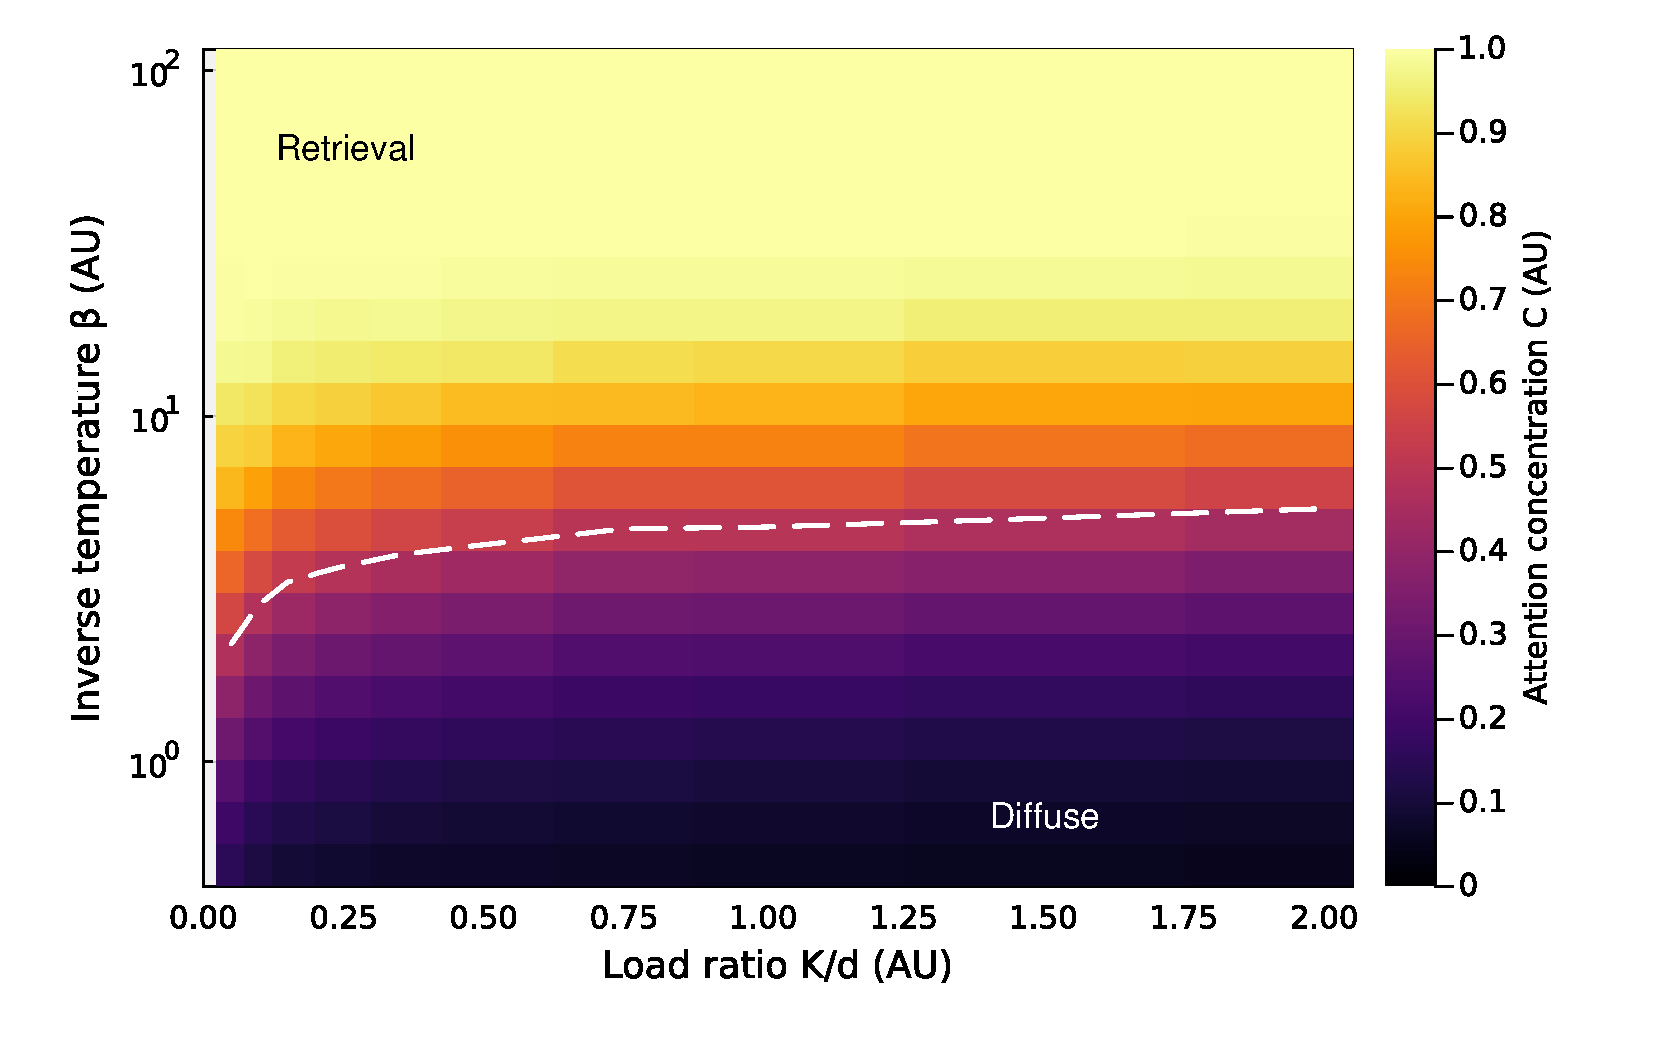
\includegraphics[width=0.65\textwidth]{figs/Fig_experiment-3-load-ratio.pdf}
\caption{Phase diagram of attention concentration $C = 1 - H(\mathbf{a})/\log K$ over load ratio $K/d$ (horizontal) and inverse temperature $\beta$ (vertical, log~scale), with $d=64$. Each cell averages over five independent datasets. The dashed contour marks $C=0.5$, separating a retrieval regime (upper-left, warm colors) from a diffuse regime (lower-right, dark colors).}
\label{fig:phase-diagram}
\end{figure}

\section{Multi-Digit MNIST Generalization}\label{app:multidigit}

To verify that the results reported for digit ``3'' in the main text are not specific to a single morphological class, we repeated the identical multi-chain protocol (30~chains, $T{=}5{,}000$, burn-in~$2{,}000$, thin every 100 then sub-sample 5, $\beta{=}2000$, $\alpha{=}0.01$, $K{=}100$ stored patterns per digit) on two additional MNIST digits chosen for their distinct morphological properties: digit ``1'' (simple stroke, near-degenerate orientation) and digit ``8'' (complex topology with two enclosed loops and high intra-class variance). All seven baselines (including the VAE) and the MALA variant were run with the identical protocol; results appear in Tables~\ref{tab:mnist-digit1} and~\ref{tab:mnist-digit8}.

\begin{table}[h]
\centering
\caption{Quantitative comparison on MNIST digit ``1'' ($K{=}100$, $d{=}784$, $\beta{=}2000$). Same protocol as Table~\ref{tab:mnist-baselines}, including the VAE baseline (latent dim 8, same two-phase training). MALA acceptance rate: 99.2\%. Values are mean $\pm$ SE across 30 chains.}
\label{tab:mnist-digit1}
\small
\begin{tabular}{@{}lccc@{}}
\toprule
Method & $\mathcal{N}$ $\uparrow$ & $\bar{\mathcal{D}}$ $\uparrow$ & $\bar{E}$ $\downarrow$ \\
\midrule
Bootstrap (replay)          & $0.000 \pm 0.000$ & $0.416 \pm 0.019$ & $-0.500 \pm 0.000$ \\
Gaussian perturbation       & $0.004 \pm 0.000$ & $0.422 \pm 0.017$ & $-0.496 \pm 0.000$ \\
Random convex combination   & $0.097 \pm 0.001$ & $0.007 \pm 0.000$ & $-0.398 \pm 0.001$ \\
GMM-PCA ($r{=}50$, $C{=}10$) & $0.130 \pm 0.005$ & $0.401 \pm 0.017$ & $-0.366 \pm 0.005$ \\
VAE (latent${=}8$)          & $0.180 \pm 0.006$ & $0.408 \pm 0.008$ & $-0.320 \pm 0.006$ \\
MALA                        & $0.151 \pm 0.001$ & $0.586 \pm 0.001$ & $-0.305 \pm 0.001$ \\
\textbf{Stochastic attention} & $\mathbf{0.153 \pm 0.001}$ & $\mathbf{0.591 \pm 0.001}$ & $\mathbf{-0.303 \pm 0.001}$ \\
\bottomrule
\end{tabular}
\end{table}

\begin{table}[h]
\centering
\caption{Quantitative comparison on MNIST digit ``8'' ($K{=}100$, $d{=}784$, $\beta{=}2000$). Same protocol as Table~\ref{tab:mnist-baselines}, including the VAE baseline (latent dim 8, same two-phase training). MALA acceptance rate: 99.2\%. Values are mean $\pm$ SE across 30 chains.}
\label{tab:mnist-digit8}
\small
\begin{tabular}{@{}lccc@{}}
\toprule
Method & $\mathcal{N}$ $\uparrow$ & $\bar{\mathcal{D}}$ $\uparrow$ & $\bar{E}$ $\downarrow$ \\
\midrule
Bootstrap (replay)          & $0.000 \pm 0.000$ & $0.421 \pm 0.012$ & $-0.500 \pm 0.000$ \\
Gaussian perturbation       & $0.004 \pm 0.000$ & $0.450 \pm 0.011$ & $-0.496 \pm 0.000$ \\
Random convex combination   & $0.099 \pm 0.000$ & $0.007 \pm 0.000$ & $-0.395 \pm 0.000$ \\
GMM-PCA ($r{=}50$, $C{=}10$) & $0.194 \pm 0.005$ & $0.420 \pm 0.011$ & $-0.305 \pm 0.005$ \\
VAE (latent${=}8$)          & $0.209 \pm 0.005$ & $0.397 \pm 0.009$ & $-0.291 \pm 0.005$ \\
MALA                        & $0.151 \pm 0.001$ & $0.554 \pm 0.002$ & $-0.305 \pm 0.001$ \\
\textbf{Stochastic attention} & $\mathbf{0.152 \pm 0.001}$ & $\mathbf{0.557 \pm 0.001}$ & $\mathbf{-0.303 \pm 0.001}$ \\
\bottomrule
\end{tabular}
\end{table}

Across all three digit classes, the stochastic attention sampler and MALA produced practically indistinguishable metrics, both dominating every baseline on diversity simultaneously. The VAE (latent dim 8) was the strongest non-Langevin baseline on novelty ($0.180$--$0.209$ vs.\ $0.130$--$0.194$ for GMM-PCA), but both learned models were far below the Langevin methods on diversity ($0.397$--$0.408$ for VAE vs.\ $0.557$--$0.600$ for SA), confirming that a static learned density cannot match the ergodic coverage of Langevin dynamics. The MALA acceptance rate was 99.2\% for all digits, confirming that ULA discretization bias remains negligible regardless of digit morphology.

Figures~\ref{fig:mnist-digit1-grids} and~\ref{fig:mnist-digit8-grids} show representative $4{\times}4$ sample grids for each method. The qualitative pattern was the same as for digit ``3'': bootstrap outputs were exact stored copies, Gaussian perturbation was visually indistinguishable from bootstrap, random convex combinations produced uniform blurry averages, and both Langevin methods generated diverse, structured digits.

\begin{figure}[h]
\centering
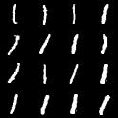
\includegraphics[width=0.19\textwidth]{figs/Fig_mnist_grid_bootstrap_digit1.png}%
\hfill
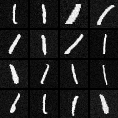
\includegraphics[width=0.19\textwidth]{figs/Fig_mnist_grid_gaussian_digit1.png}%
\hfill
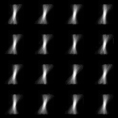
\includegraphics[width=0.19\textwidth]{figs/Fig_mnist_grid_convex_digit1.png}%
\hfill
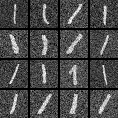
\includegraphics[width=0.19\textwidth]{figs/Fig_mnist_grid_mala_digit1.png}%
\hfill
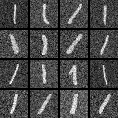
\includegraphics[width=0.19\textwidth]{figs/Fig_mnist_grid_sa_digit1.png}

\small
\makebox[0.19\textwidth]{\centering (a) Bootstrap}%
\hfill
\makebox[0.19\textwidth]{\centering (b) Gaussian}%
\hfill
\makebox[0.19\textwidth]{\centering (c) Convex}%
\hfill
\makebox[0.19\textwidth]{\centering (d) MALA}%
\hfill
\makebox[0.19\textwidth]{\centering (e) Ours}
\caption{Generated MNIST digit ``1'' samples ($4{\times}4$ grids). The pattern matches digit ``3'': only the Langevin-based methods (d,\,e) produce diverse, structured outputs.}
\label{fig:mnist-digit1-grids}
\end{figure}

\begin{figure}[h]
\centering
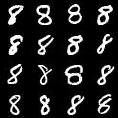
\includegraphics[width=0.19\textwidth]{figs/Fig_mnist_grid_bootstrap_digit8.png}%
\hfill
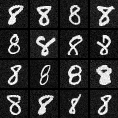
\includegraphics[width=0.19\textwidth]{figs/Fig_mnist_grid_gaussian_digit8.png}%
\hfill
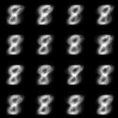
\includegraphics[width=0.19\textwidth]{figs/Fig_mnist_grid_convex_digit8.png}%
\hfill
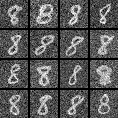
\includegraphics[width=0.19\textwidth]{figs/Fig_mnist_grid_mala_digit8.png}%
\hfill
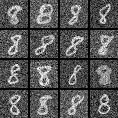
\includegraphics[width=0.19\textwidth]{figs/Fig_mnist_grid_sa_digit8.png}

\small
\makebox[0.19\textwidth]{\centering (a) Bootstrap}%
\hfill
\makebox[0.19\textwidth]{\centering (b) Gaussian}%
\hfill
\makebox[0.19\textwidth]{\centering (c) Convex}%
\hfill
\makebox[0.19\textwidth]{\centering (d) MALA}%
\hfill
\makebox[0.19\textwidth]{\centering (e) Ours}
\caption{Generated MNIST digit ``8'' samples ($4{\times}4$ grids). Despite digit ``8'' having higher intra-class variance and more complex topology than digit ``3'', the qualitative pattern is unchanged: Langevin methods dominate all baselines.}
\label{fig:mnist-digit8-grids}
\end{figure}

\paragraph{Temperature spectrum on digit ``8.''}
The baseline comparison above fixes $\beta{=}2000$, which places the sampler deep in the retrieval regime: each chain stays near its seed pattern and the ``generation'' is local variation within a single energy basin.
To show the full retrieval-generation trade-off on real images, Figure~\ref{fig:temp-spectrum-digit8} displays $4{\times}4$ SA grids at four inverse temperatures alongside 16 stored patterns for reference.
Table~\ref{tab:temp-spectrum-digit8} reports the corresponding metrics.

\begin{table}[h]
\centering
\caption{Temperature spectrum for digit ``8'' ($K{=}100$, $d{=}784$, $\alpha{=}0.01$, 30 chains). $\mathrm{SNR}=\sqrt{\alpha\beta/2d}$ is the per-step signal-to-noise ratio; the transition occurs near $\mathrm{SNR}^{*}=\sqrt{\alpha/(2\sqrt{d})}$ (Proposition~\ref{prop:entropy-derivative}); at $d{=}784$ and $\alpha{=}0.01$ this gives $\mathrm{SNR}^{*}\approx 0.013$. As SNR falls through this region the sampler crosses from structured retrieval into diffuse generation. Values are mean $\pm$ SE across 30 chains.}
\label{tab:temp-spectrum-digit8}
\small
\begin{tabular}{@{}rccccc@{}}
\toprule
$\beta$ & SNR & $\mathcal{N}$ $\uparrow$ & $\bar{\mathcal{D}}$ $\uparrow$ & $\bar{E}$ $\downarrow$ & Mean max-$\cos$ \\
\midrule
2000 & 0.113 & $0.152 \pm 0.001$ & $0.557 \pm 0.001$ & $-0.3 \pm 0.00$ & $0.848 \pm 0.001$ \\
200  & 0.036 & $0.547 \pm 0.002$ & $0.872 \pm 0.002$ & $1.5 \pm 0.01$  & $0.453 \pm 0.002$ \\
50   & 0.018 & $0.753 \pm 0.002$ & $0.965 \pm 0.002$ & $7.4 \pm 0.03$  & $0.247 \pm 0.002$ \\
10   & 0.008 & $0.870 \pm 0.003$ & $0.992 \pm 0.002$ & $38.6 \pm 0.16$ & $0.130 \pm 0.003$ \\
\bottomrule
\end{tabular}
\end{table}

At $\beta{=}2000$ the outputs were recognizable eights that closely resembled individual stored patterns (mean max-cos 0.85); novelty was low and diversity came entirely from the multi-chain initialization, not from any single chain exploring between basins.
As $\beta$ decreased, the energy barriers shrank, chains escaped their initial basins, and novelty/diversity rose sharply.
At $\beta{=}200$ the mean max-cosine dropped to 0.45, meaning outputs sat roughly halfway between stored patterns, a regime of genuine interpolation.
By $\beta{=}50$ the samples were highly novel (0.75) but began to lose recognizable digit structure, and at $\beta{=}10$ the outputs were essentially isotropic noise with no visual resemblance to eights.
This illustrates the fundamental retrieval-generation trade-off: no single $\beta$ simultaneously maximizes fidelity and novelty. The operating point must be chosen according to the application, and the temperature parameter gives the user explicit control over this trade-off.

\begin{figure}[h]
\centering
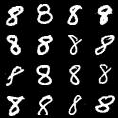
\includegraphics[width=0.19\textwidth]{figs/Fig_mnist_tempspectrum_digit8_stored.png}%
\hfill
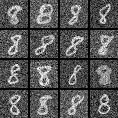
\includegraphics[width=0.19\textwidth]{figs/Fig_mnist_tempspectrum_digit8_beta2000.png}%
\hfill
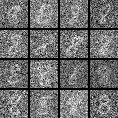
\includegraphics[width=0.19\textwidth]{figs/Fig_mnist_tempspectrum_digit8_beta200.png}%
\hfill
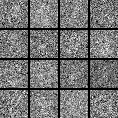
\includegraphics[width=0.19\textwidth]{figs/Fig_mnist_tempspectrum_digit8_beta50.png}%
\hfill
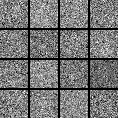
\includegraphics[width=0.19\textwidth]{figs/Fig_mnist_tempspectrum_digit8_beta10.png}

\small
\makebox[0.19\textwidth]{\centering Stored}%
\hfill
\makebox[0.19\textwidth]{\centering $\beta{=}2000$}%
\hfill
\makebox[0.19\textwidth]{\centering $\beta{=}200$}%
\hfill
\makebox[0.19\textwidth]{\centering $\beta{=}50$}%
\hfill
\makebox[0.19\textwidth]{\centering $\beta{=}10$}
\caption{Temperature spectrum for MNIST digit ``8.'' From left to right: 16 stored patterns; SA samples at $\beta{=}2000$ (retrieval, local variation around stored patterns); $\beta{=}200$ (intermediate, genuine interpolation); $\beta{=}50$ (high novelty, structure fading); $\beta{=}10$ (diffuse noise). The trade-off between fidelity and novelty is governed entirely by~$\beta$.}
\label{fig:temp-spectrum-digit8}
\end{figure}

\section{Single-Chain Diversity Analysis}\label{app:single-chain}

Table~\ref{tab:mnist-baselines} uses 30 independent chains each initialized near a different stored pattern; the reported diversity of $0.600$ includes both \emph{initialization diversity} (spread from 30 distinct seeds) and \emph{within-chain mixing} (sampling from a fixed starting point). To quantify these contributions separately, we ran one chain from a fixed initialization (stored pattern~1 plus $\sigma_{\mathrm{init}}{=}0.01$ Gaussian noise, seed fixed) for $T{=}50{,}000$ steps (burn-in $10{,}000$, thin every~100, yielding 400 samples) at $\beta\in\{2000,\,200,\,50\}$ ($\mathrm{SNR}\in\{0.113,\,0.036,\,0.018\}$) on digit~``3''.

\begin{table}[h]
\centering
\caption{Single-chain vs.\ multi-chain diversity on digit ``3'' ($K{=}100$, $d{=}784$, $\alpha{=}0.01$). $\mathrm{SNR}=\sqrt{\alpha\beta/2d}$. The multi-chain row reproduces the SA entry from Table~\ref{tab:mnist-baselines}. The diversity gap of $0.318$ at $\mathrm{SNR}{=}0.113$ is the initialization contribution; single-chain diversity exceeds the multi-chain value once SNR falls toward the entropy inflection point (Proposition~\ref{prop:entropy-derivative}).}
\label{tab:single-chain}
\small
\begin{tabular}{@{}llccccc@{}}
\toprule
Protocol & $\beta$ & SNR & $\mathcal{N}$ $\uparrow$ & $\bar{\mathcal{D}}$ $\uparrow$ & $\bar{E}$ $\downarrow$ & Max-$\cos$ \\
\midrule
Multi-chain (30 chains) & 2000 & 0.113 & $0.152 \pm 0.001$ & $0.600 \pm 0.001$ & $-0.303 \pm 0.001$ & $0.848 \pm 0.001$ \\
Single-chain            & 2000 & 0.113 & $0.153 \pm 0.000$ & $0.282 \pm 0.001$ & $-0.300 \pm 0.000$ & $0.847 \pm 0.000$ \\
Single-chain            & 200  & 0.036 & $0.551 \pm 0.001$ & $0.796 \pm 0.002$ & $\phantom{-}1.5\phantom{0} \pm 0.0\phantom{0}$ & $0.449 \pm 0.001$ \\
Single-chain            & 50   & 0.018 & $0.756 \pm 0.002$ & $0.967 \pm 0.002$ & $\phantom{-}7.4\phantom{0} \pm 0.0\phantom{0}$ & $0.244 \pm 0.002$ \\
\bottomrule
\end{tabular}
\end{table}

\begin{figure}[h]
\centering
\begin{minipage}[t]{0.31\textwidth}
\centering
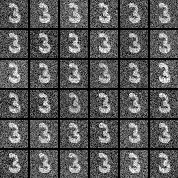
\includegraphics[width=\linewidth]{figs/Fig_single_chain_grid_beta2000.png}\\[-2pt]
\small (a) $\beta{=}2000$, SNR$=0.113$\\structured retrieval ($\bar{\mathcal{D}}{=}0.282$)
\end{minipage}
\hfill
\begin{minipage}[t]{0.31\textwidth}
\centering
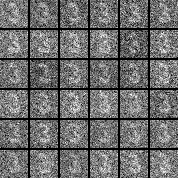
\includegraphics[width=\linewidth]{figs/Fig_single_chain_grid_beta200.png}\\[-2pt]
\small (b) $\beta{=}200$, SNR$=0.036$\\genuine generation ($\bar{\mathcal{D}}{=}0.796$)
\end{minipage}
\hfill
\begin{minipage}[t]{0.31\textwidth}
\centering
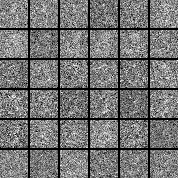
\includegraphics[width=\linewidth]{figs/Fig_single_chain_grid_beta50.png}\\[-2pt]
\small (c) $\beta{=}50$, SNR$=0.018$\\diffuse ($\bar{\mathcal{D}}{=}0.967$)
\end{minipage}
\caption{Single-chain samples ($6{\times}6$ grids, digit ``3'') from a fixed seed at three operating points. \textbf{(a)}~At SNR$=0.113$ the chain stays near one stored pattern; diversity is low ($0.282$). \textbf{(b)}~At SNR$=0.036$ the chain spontaneously crosses energy barriers; single-chain diversity ($0.796$) \emph{exceeds} the 30-chain $\beta{=}2000$ value ($0.600$), confirming genuine generation. \textbf{(c)}~At SNR$=0.018$ the chain is fully diffuse; samples lose recognizable digit structure.}
\label{fig:generation-regimes}
\end{figure}

At $\beta{=}2000$ the single-chain diversity of $0.282$ is not negligible: the chain samples a genuine distribution within its energy basin rather than collapsing to a point mass. As $\beta$ decreased the energy barriers shrank, chains escaped their initial basins, and single-chain diversity rose sharply, mirroring the temperature-spectrum results of Appendix~\ref{app:multidigit}. At $\beta{=}200$ single-chain diversity ($0.796$) exceeds the multi-chain value at $\beta{=}2000$, and at $\beta{=}50$ it approaches the isotropic limit ($0.967$, mean max-cos $0.244$). The multi-chain protocol at $\beta{=}2000$ is therefore best understood as a \emph{structured retrieval} strategy in which each chain contributes low-energy samples from a distinct basin, while single-chain operation at $\beta{=}200$ provides genuine generative diversity without requiring multiple initializations.

\paragraph{Mixing time.}
At $\beta{=}2000$ the single chain remained in the basin of its seed pattern for the entire $50{,}000$-step run (${\approx}12$\,s wall-clock on a laptop CPU): the max-cosine to the seed pattern stayed above $0.84$ at every thinned sample, and the chain never visited the basin of any other stored pattern. The \emph{inter-basin} mixing time at this temperature therefore exceeds $50{,}000$ steps, consistent with the exponential-barrier scaling discussed in Section~4. \emph{Intra-basin} mixing, by contrast, is fast: energy and max-cosine stabilize within the $2{,}000$-step burn-in, and consecutive thinned samples (every $100$ steps) have pairwise cosine distance $0.11\pm0.01$, indicating decorrelation within $O(100)$ steps. At $\beta{=}200$ the picture changes: the chain crosses into a different basin within the first ${\approx}5{,}000$ steps and visits multiple basins over the $50{,}000$-step run, yielding the observed single-chain diversity of $0.796$.

% ─────────────────────────────────────────────────────────────────────────────
\section{Protein Sequence Generation}\label{app:protein}
% ─────────────────────────────────────────────────────────────────────────────

To test stochastic attention on a non-image domain with discrete structure, we applied the full experimental pipeline to protein sequences from the Pfam RRM family (PF00076, RNA Recognition Motif)~\cite{mistryPfamProteinFamilies2021}.

\paragraph{Data and encoding.}
We downloaded the Pfam seed alignment (Stockholm format), removed columns with $>50\%$ gaps and sequences with $>30\%$ gaps, yielding $K{=}68$ aligned sequences of length $L{=}71$ positions over the 20 standard amino acids. Each sequence was one-hot encoded into $\mathbb{R}^{1420}$ ($20\times 71$), projected via PCA retaining 95\% of variance ($1420\to 59$ dimensions), and $\ell_2$-normalized to form the memory matrix $\hat{\mathbf{X}}\in\mathbb{R}^{59\times 68}$.

\paragraph{Phase transition.}
The entropy inflection analysis (Proposition~\ref{prop:entropy-derivative}) yielded $\beta^*\approx 3.85$ ($\mathrm{SNR}^*=0.018$), compared to the theoretical prediction $\beta^*=\sqrt{d}=7.68$ for random unit-norm patterns. The ratio of $0.50$ reflects the structured (non-random) geometry of the protein family: conserved positions reduce the effective variance of the similarities $e_k$, shifting the transition to lower $\beta$. We set $\beta_{\mathrm{ret}}=20\beta^*\approx 77$ ($\mathrm{SNR}=0.081$) for the structured-retrieval regime and $\beta_{\mathrm{gen}}=2\beta^*\approx 8$ ($\mathrm{SNR}=0.026$, just above the inflection) for the generation regime.

\paragraph{Protocol.}
We ran the identical multi-chain protocol used for MNIST: 30 chains, $T{=}5{,}000$ iterations, burn-in $2{,}000$, thinning every 100 steps, 5 samples per chain, yielding $S{=}150$ generated sequences. SA was run at both $\beta_{\mathrm{ret}}{=}77$ (retrieval) and $\beta_{\mathrm{gen}}{=}8$ (generation) to demonstrate the temperature knob on a non-image domain. All seven baselines (bootstrap, Gaussian perturbation, random convex combination, GMM-PCA, VAE with latent dim 8, MALA) were run with the same protocol. Generated PCA-space vectors were decoded back to amino acid sequences by inverse-PCA followed by per-position argmax over the 20 amino acid channels.

\paragraph{Metrics.}
In addition to the standard metrics (novelty~$\mathcal{N}$, diversity~$\bar{\mathcal{D}}$, energy~$\bar{E}$), we report two protein-specific measures: \emph{sequence identity} to the nearest stored member (max over stored sequences of the fraction of non-gap positions with matching amino acids) and \emph{amino acid composition KL divergence} ($D_{\mathrm{KL}}(p_{\mathrm{stored}}\|q_{\mathrm{gen}})$ over the 20 amino acid frequencies).

\begin{table}[h]
\centering
\caption{Protein sequence generation on Pfam PF00076 (RRM family, $K{=}68$, $L{=}71$, $d{=}59$ after PCA). Two SA rows demonstrate the temperature knob: $\beta{=}77$ (retrieval, $20\beta^*$) and $\beta{=}8$ (generation, $2\beta^*$). SeqID: maximum sequence identity to any stored sequence. KL: amino acid composition divergence from stored sequences (lower is better). $^\dagger$Energy is positive at $\beta{=}8$ because samples explore off the attractor manifold. MALA acceptance rate: 99.8\%.}
\label{tab:protein}
\small
\begin{tabular}{@{}lccccc@{}}
\toprule
Method & $\mathcal{N}$ $\uparrow$ & $\bar{\mathcal{D}}$ $\uparrow$ & $\bar{E}$ $\downarrow$ & SeqID & KL $\downarrow$ \\
\midrule
Bootstrap (replay)          & $0.000 \pm 0.000$ & $1.000 \pm 0.012$ & $-0.500 \pm 0.000$ & $0.645 \pm 0.004$ & 0.133 \\
Gaussian perturbation       & $0.008 \pm 0.000$ & $1.002 \pm 0.007$ & $-0.492 \pm 0.000$ & $0.633 \pm 0.006$ & 0.132 \\
Random convex combination   & $0.510 \pm 0.009$ & $0.994 \pm 0.009$ & $-0.068 \pm 0.001$ & $0.562 \pm 0.000$ & 2.091 \\
GMM-PCA ($r{=}50$, $C{=}10$) & $0.606 \pm 0.009$ & $1.000 \pm 0.007$ & $+0.077 \pm 0.009$ & $0.540 \pm 0.003$ & 0.731 \\
VAE (latent${=}8$)          & $0.621 \pm 0.007$ & $0.834 \pm 0.022$ & $+0.118 \pm 0.007$ & $0.532 \pm 0.003$ & 0.416 \\
MALA ($\beta{=}77$)         & $0.249 \pm 0.004$ & $0.992 \pm 0.007$ & $-0.115 \pm 0.005$ & $0.609 \pm 0.012$ & 0.112 \\
SA ($\beta{=}77$, retrieval) & $0.243 \pm 0.004$ & $0.991 \pm 0.007$ & $-0.120 \pm 0.006$ & $0.616 \pm 0.012$ & 0.107 \\
\textbf{SA ($\beta{=}8$, generation)} & $\mathbf{0.623 \pm 0.006}$ & $\mathbf{1.001 \pm 0.006}$ & $3.08 \pm 0.06^\dagger$ & $\mathbf{0.538 \pm 0.006}$ & \textbf{0.060} \\
\bottomrule
\end{tabular}
\end{table}

\begin{figure}[h]
\centering
\begin{minipage}[t]{0.48\textwidth}
\centering
\IfFileExists{figs/Fig_protein_aa_frequencies.pdf}{%
  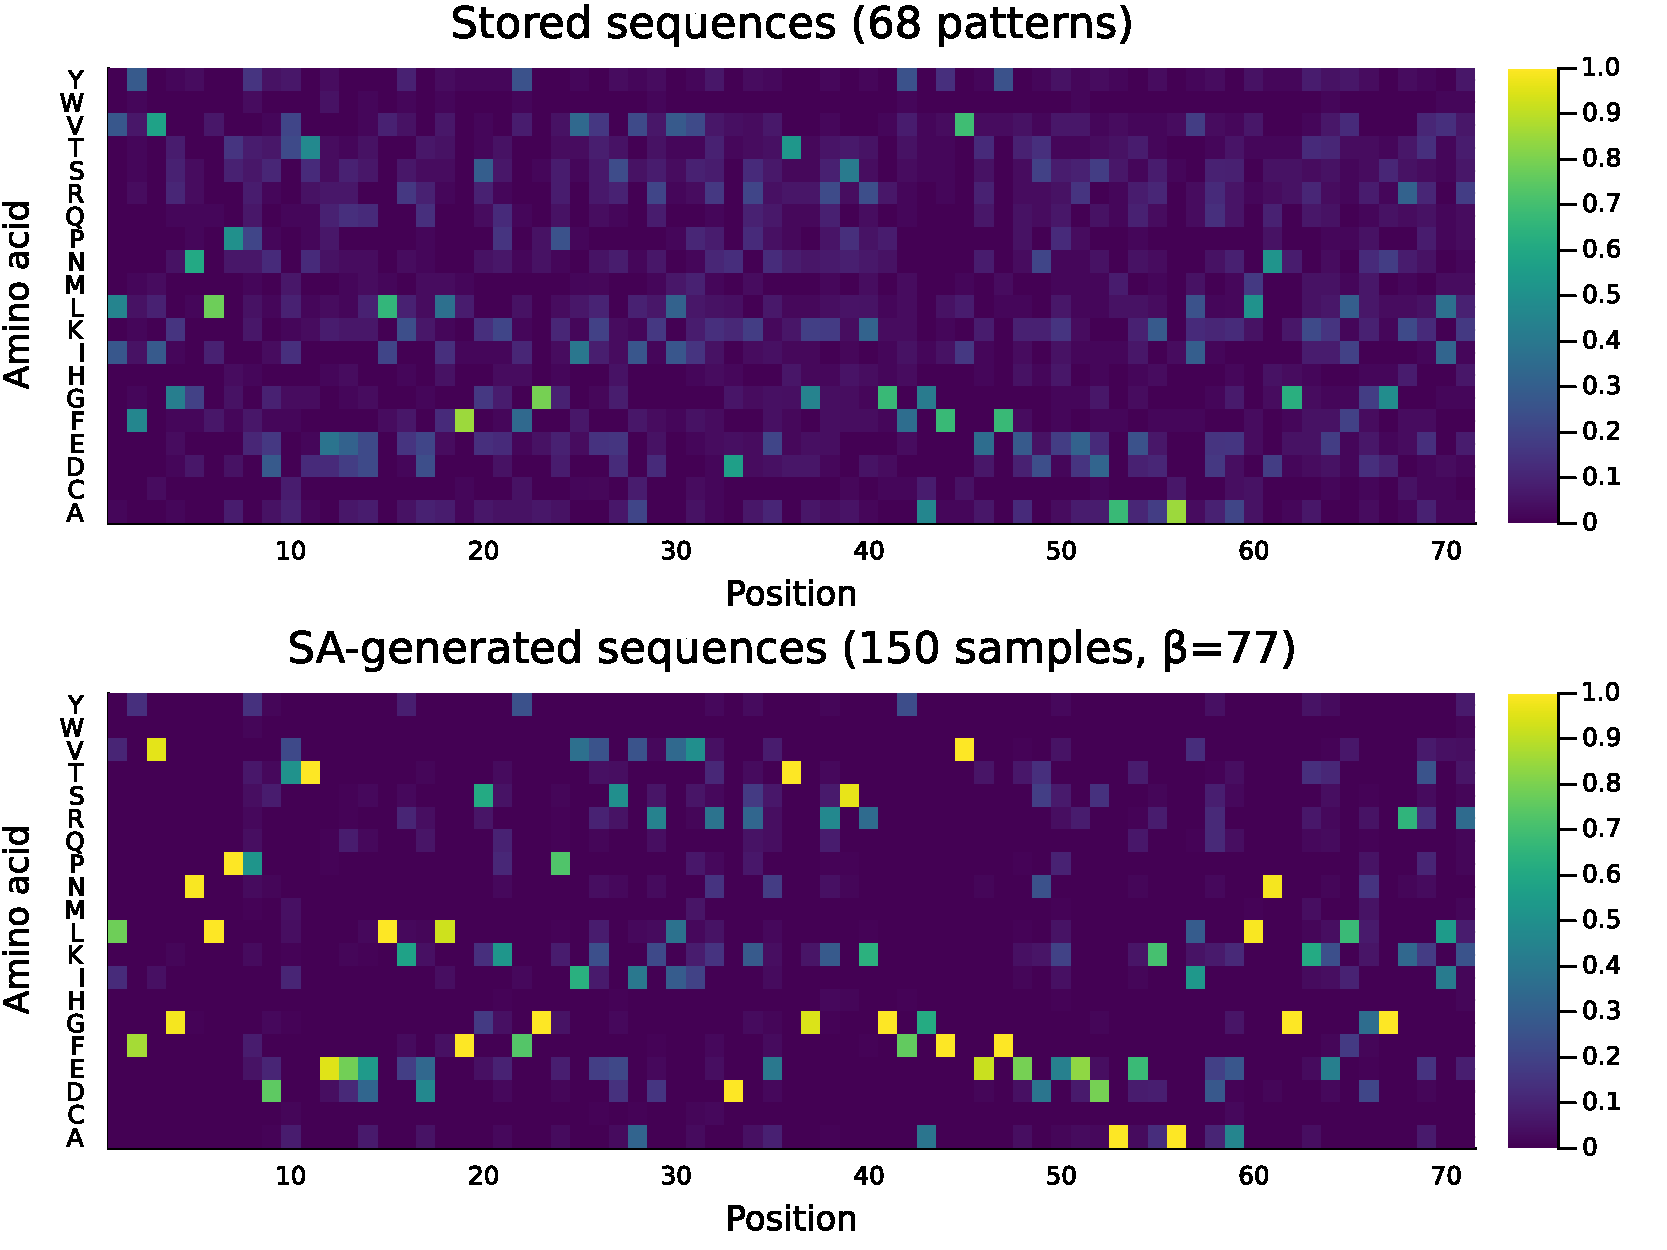
\includegraphics[width=\linewidth]{figs/Fig_protein_aa_frequencies.pdf}%
}{%
  \framebox[\linewidth]{\rule{0pt}{4cm}\small [AA frequency heatmap]}%
}
\end{minipage}
\hfill
\begin{minipage}[t]{0.48\textwidth}
\centering
\IfFileExists{figs/Fig_protein_sequence_identity.pdf}{%
  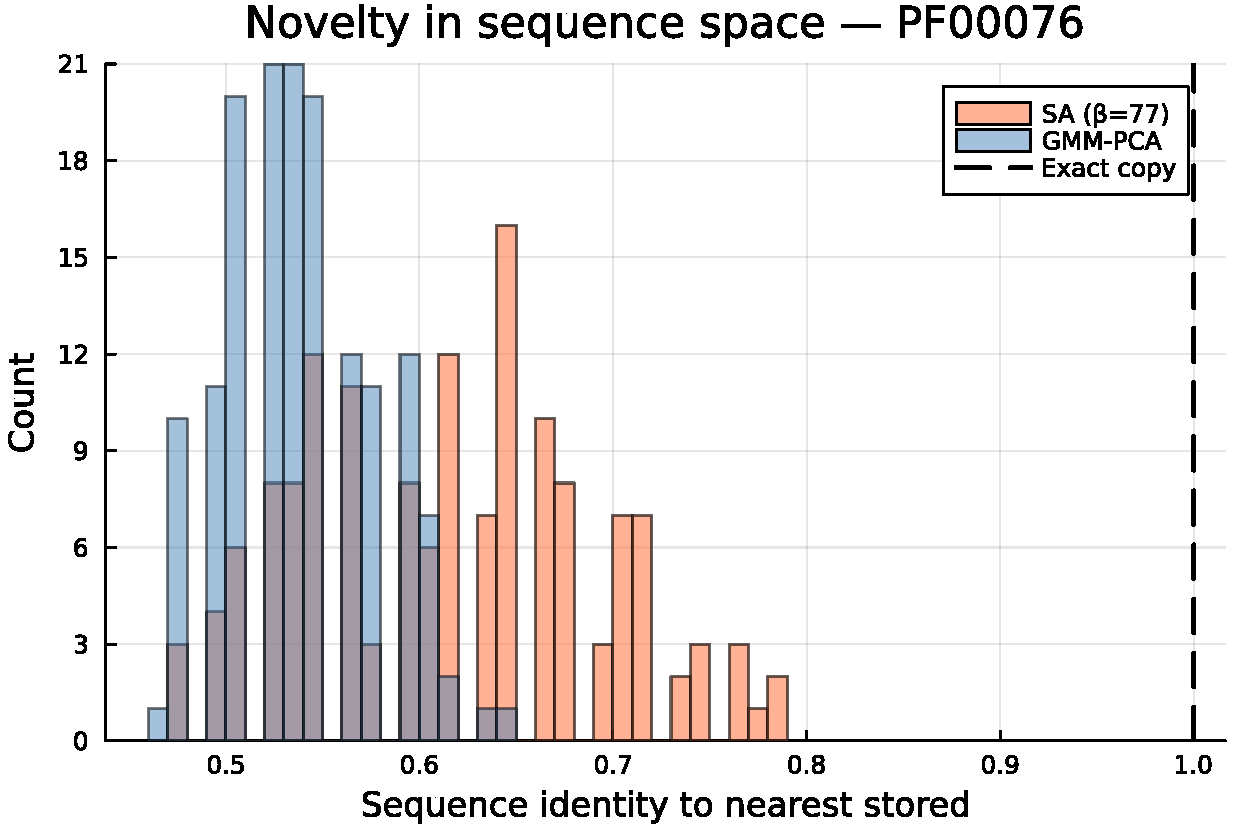
\includegraphics[width=\linewidth]{figs/Fig_protein_sequence_identity.pdf}%
}{%
  \framebox[\linewidth]{\rule{0pt}{4cm}\small [Sequence identity histogram]}%
}
\end{minipage}
\caption{Protein sequence generation on PF00076. \textbf{Left:} Per-position amino acid frequencies for stored sequences (top) and SA-generated sequences (bottom). SA preserves the conserved positions of the RRM family while introducing variation at non-conserved sites. \textbf{Right:} Distribution of sequence identity to the nearest stored member for SA and GMM-PCA. SA generates sequences that are ${\approx}62\%$ identical to their nearest stored neighbor, while GMM-PCA produces more distant sequences (${\approx}54\%$) with much higher compositional divergence (KL$=0.731$ vs.\ $0.107$).}
\label{fig:protein}
\end{figure}

Table~\ref{tab:protein} reveals the same two-regime structure observed on MNIST. At $\beta{=}77$ (retrieval), SA generates sequences ${\approx}62\%$ identical to their nearest stored member with the lowest KL divergence of any method at this temperature ($0.107$). SA and MALA are again indistinguishable (MALA acceptance $99.8\%$), consistent with the MNIST results. Random convex combinations catastrophically distort the composition (KL$=2.091$) because averaging one-hot vectors in PCA space does not preserve per-position amino acid structure.

At $\beta{=}8$ (generation, $2\beta^*$), SA matches the VAE on novelty ($0.623$ vs.\ $0.621$) and exceeds it on diversity ($1.001$ vs.\ $0.834$), while achieving dramatically lower compositional divergence: KL$=0.060$ vs.\ $0.416$ for the VAE, a $6.9{\times}$ improvement. This means SA-generated sequences at generation temperature have the closest amino acid composition to the real RRM family of any method tested, including all baselines and SA at retrieval temperature. The temperature knob works as designed: lowering $\beta$ from retrieval to generation trades sequence identity ($0.616\to 0.538$) for novelty ($0.243\to 0.623$) while preserving family-level compositional fidelity. Energy rises above zero (samples leave the attractor manifold), but the Langevin gradient keeps the chain closer to the memory geometry than any learned baseline.

The entropy inflection analysis validates at this new dimensionality: the empirical $\beta^*{=}3.85$ is approximately half the random-pattern prediction $\sqrt{d}{=}7.68$ (Fig.~\ref{fig:protein-entropy}). This discrepancy is expected: RRM sequences share conserved residues at many positions, reducing the effective variance of the query-key similarities and shifting the phase transition to lower $\beta$. The inflection criterion (Eq.~\ref{eq:inflection}) automatically accounts for this structure, providing the correct operating point without manual tuning.

\begin{figure}[h]
\centering
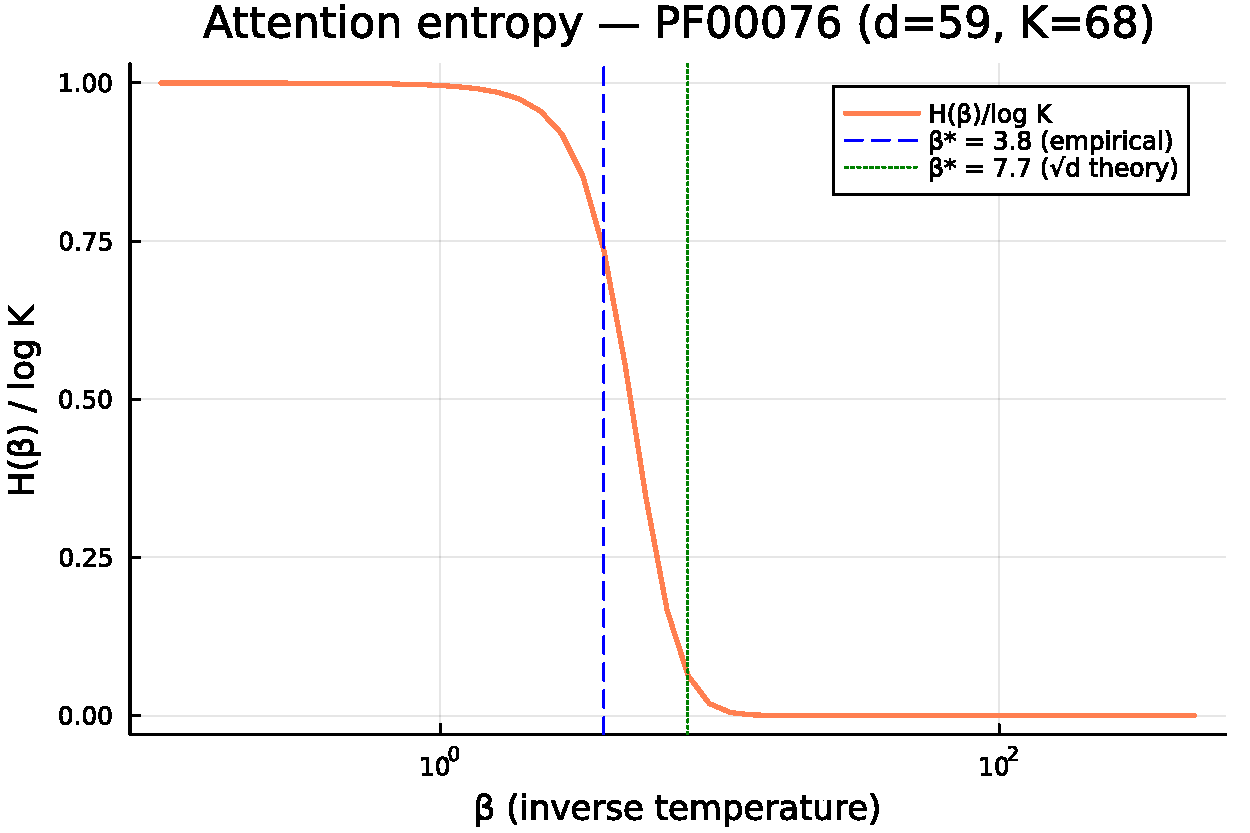
\includegraphics[width=0.55\textwidth]{figs/Fig_protein_entropy_curve.pdf}
\caption{Attention entropy $H(\beta)/\log K$ for the Pfam RRM memory ($K{=}68$, $d{=}59$). The empirical inflection point $\beta^*{=}3.8$ (dashed blue) occurs at roughly half the random-pattern prediction $\sqrt{d}{=}7.7$ (dotted green), reflecting the reduced effective similarity variance caused by conserved residues.}
\label{fig:protein-entropy}
\end{figure}

\paragraph{HMMER validation.}
To provide a biologically meaningful validity metric beyond amino acid composition, we validated all generated sequences against the Pfam RRM profile HMM using HMMER~3.4~\cite{hmmer3}. Gap characters were removed from each generated sequence before submission to \texttt{hmmsearch}. All $150$ generated sequences from every method pass at $E$-value~$<0.01$, with SA at generation temperature achieving a median $E$-value of $8.1{\times}10^{-34}$ -- far below the threshold and lower (better) than the stored sequences' median of $2.5{\times}10^{-22}$. The generated sequences achieve better $E$-values because the generation process produces smoother, more canonical sequences that match the HMM consensus closely. The $100\%$ pass rate confirms that SA-generated sequences are biologically valid RRM family members, not arbitrary sequences that happen to share amino acid composition statistics.

\paragraph{Position-specific fidelity.}
The global amino acid KL divergence aggregates frequencies across all positions. To verify that SA preserves \emph{position-specific} conservation patterns, we computed the KL divergence independently at each of the $L{=}71$ aligned positions and report the mean.

SA in the generation regime achieves a mean per-position KL of $2.92$, compared to $9.99$ for the VAE ($3.4{\times}$ lower), $7.52$ for bootstrap, and $9.09$ for GMM-PCA. This confirms that the advantage extends beyond global composition to position-specific conservation patterns: SA correctly identifies which positions are conserved and which are variable, preserving the position-specific amino acid distribution at each residue. MALA at generation temperature achieves a comparable $2.96$.

\paragraph{Pairwise coupling fidelity.}
To address the concern that marginal frequency metrics ignore sequence-level dependencies, we computed the pairwise mutual information (MI) between residue positions. For a set of sequences, the MI between positions $i$ and $j$ is $\mathrm{MI}(i,j)=\sum_{a,b}p(a,b)\log\bigl[p(a,b)/(p(a)p(b))\bigr]$, where $p(a,b)$ is the joint frequency of amino acids $a$ and $b$ at positions $i$ and $j$. We computed MI matrices for each method's generated sequences and measured the Pearson correlation with the stored family's MI matrix.

SA at generation temperature achieves MI correlation $r{=}0.871$, compared to $r{=}0.525$ for the VAE -- a $66\%$ improvement. Bootstrap replay achieves $r{=}0.692$ and SA at retrieval temperature achieves $r{=}0.733$. This demonstrates that SA-generated sequences reproduce the pairwise co-evolutionary coupling structure of the RRM family, capturing sequence-level dependencies that go beyond single-position statistics. The high MI correlation, combined with the low per-position KL and $100\%$ HMM pass rate, provides strong evidence that SA-generated sequences are structurally and functionally plausible RRM family members.

\paragraph{MALA at generation temperature.}
SA and MALA produce near-identical results at the generation temperature ($\beta{=}8$): KL$=0.060$ vs.\ $0.058$, sequence identity $0.538$ vs.\ $0.537$, novelty $0.623$ vs.\ $0.616$, MI correlation $0.871$ vs.\ $0.887$ (MALA acceptance $99.8\%$). The ULA bias is negligible for protein sequences at both retrieval and generation temperatures.

\section{Financial Log-Return Generation}\label{app:finance}

The synthetic experiments validated the sampler on controlled geometry; this section used real financial data to \emph{precisely characterize} what equilibrium Boltzmann sampling on the Hopfield energy captures and, equally importantly, what it cannot, and why each limitation is a principled theoretical consequence rather than a tuning failure.

\subsection{Data and Memory Construction}

We collected daily adjusted closing prices for $d=424$ S\&P~500 constituents with complete histories over a $K=2{,}766$-trading-day window. For each firm $i$ and day $t$, the continuously compounded growth rate is $g^{(i)}_t = \log(S^{(i)}_t / S^{(i)}_{t-1})$. Each trading day yielded a $d$-dimensional return vector $\mathbf{g}_t \in \mathbb{R}^{424}$. We stored these as columns of a raw memory matrix $\mathbf{M}\in\mathbb{R}^{d\times K}$ and constructed the scaled memory matrix $\mathbf{X}\in\mathbb{R}^{d\times K}$ by centering each column to zero cross-sectional mean and normalizing to unit $\ell_2$~norm, following the standard protocol for modern Hopfield networks~\cite{ramsauerHopfieldNetworksAll2021}. The load ratio was $K/d \approx 6.5$.

\subsection{I.I.D.\ Pool: Marginal and Cross-Sectional Fidelity}

We compared SA to \emph{historical bootstrap resampling} (drawing stored return vectors uniformly at random from $\mathbf{M}$) on marginal and cross-sectional metrics. Because the projection $\hat{\mathbf{g}}=\mathbf{M}\,\operatorname{softmax}(\beta\,\mathbf{X}^\top\boldsymbol{\xi})$ is a convex combination of historical return vectors, bootstrap sets an upper bound on distributional fidelity; the key question is what SA contributes beyond verbatim replay. We launched $n_{\text{chains}}=30$ independent ULA chains, each initialized near a randomly chosen stored memory, and ran $T=5{,}000$ steps with step size $\alpha=0.01$ and fixed inverse temperature $\beta=25$ ($\mathrm{SNR}=\sqrt{\alpha\beta/2d}\approx 0.017$). After discarding a burn-in of $2{,}000$ steps and thinning every $100$, we obtained $900$ approximately i.i.d.\ samples.

\paragraph{Marginal distributions and novelty.}
For each of $d=424$ tickers, we ran a two-sample KS test between generated and historical returns, and QQ plots for five representative tickers (Figure~\ref{fig:finance-qq}). The convex-combination projection compresses per-ticker standard deviation by $\approx1.14\times$ at $\beta{=}25$ (SNR$\approx$0.017); we correct for this by applying a per-ticker affine standardization (aligning the mean and standard deviation of each ticker's generated series to the historical moments, analogous to the marginal-calibration step in copula-based scenario generation), which leaves the chain dynamics and novelty metric unchanged. After correction, $272$ of $424$ tickers pass the two-sample KS test at the $5\%$ level (mean $p{=}0.193$). Bootstrap achieves $99.3\%$ pass by drawing from the empirical distribution (mean $p{=}0.622$); the residual $35.8\%$ SA failure reflects higher-order distributional differences (skewness, kurtosis) beyond what affine correction addresses. The key distinction remains novelty: SA chain states have $1-\max_k\cos(\boldsymbol{\xi},\mathbf{X}_{:,k})=0.768\pm0.001$, while every bootstrap draw is a verbatim historical scenario (novelty~$0.000$, Table~\ref{tab:finance-summary}).

\paragraph{Cross-asset correlation.}
Figure~\ref{fig:finance-correlation} plots each of the $\binom{424}{2}=89{,}676$ pairwise correlations of the generated returns against the corresponding historical correlations. The cloud lay along the $y=x$ diagonal: SA Frobenius correlation error is $26.3\%$ versus $15.6\%$ for bootstrap. The per-ticker affine correction does not alter this value: correlation is scale-invariant, so rescaling each ticker's series preserves $\operatorname{cor}(\hat{\mathbf{G}})$ exactly. SA trades some correlation fidelity for novelty; the Hopfield energy concentrates sampling on energetically favorable regime interpolations rather than uniform historical replay.

\paragraph{Tail survival functions.}
Figure~\ref{fig:finance-tails} displays the empirical survival functions of portfolio-level (equal-weight) returns. Both right and left tails matched closely on a log scale, demonstrating that the sampler reproduced the heavy-tailed nature of equity returns without distributional assumptions.

\begin{figure}[h]
\centering
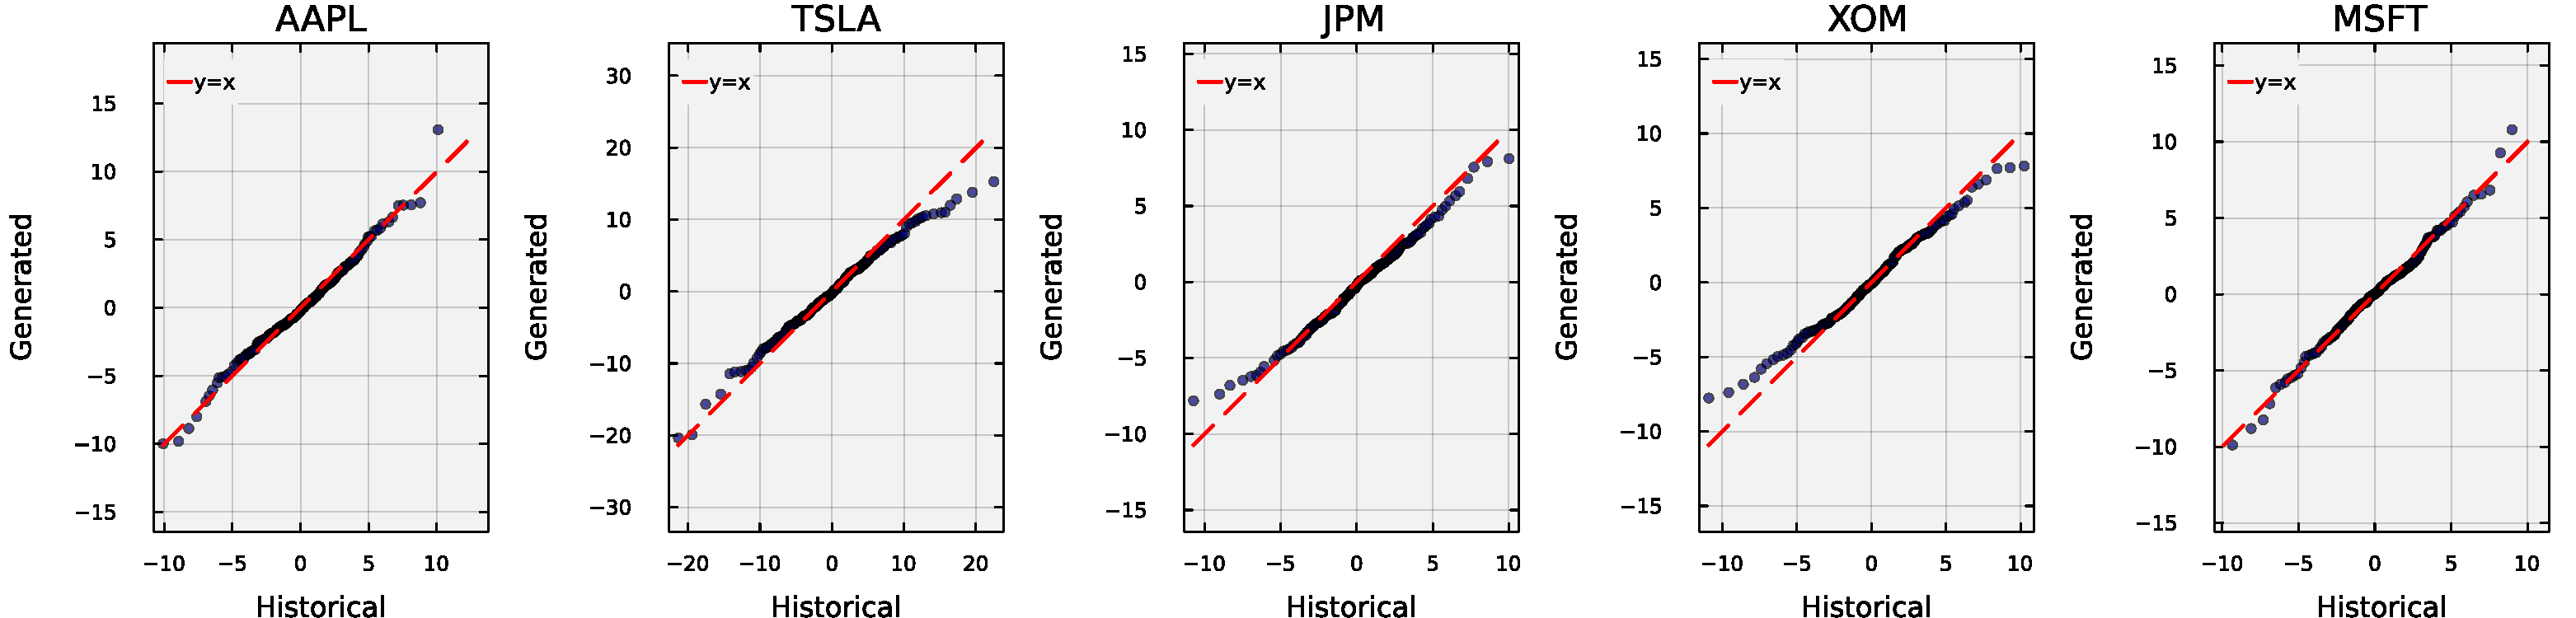
\includegraphics[width=0.95\textwidth]{figs/Fig_finance_qq_plots.pdf}
\caption{QQ plots of generated (after per-ticker affine correction) vs.\ historical log returns for five representative S\&P~500 constituents. Quantiles track closely for these tickers; $64.2\%$ of all $424$ tickers pass the two-sample KS test at the $5\%$ level. The dashed red line is $y=x$.}
\label{fig:finance-qq}
\end{figure}

\begin{figure}[h]
\centering
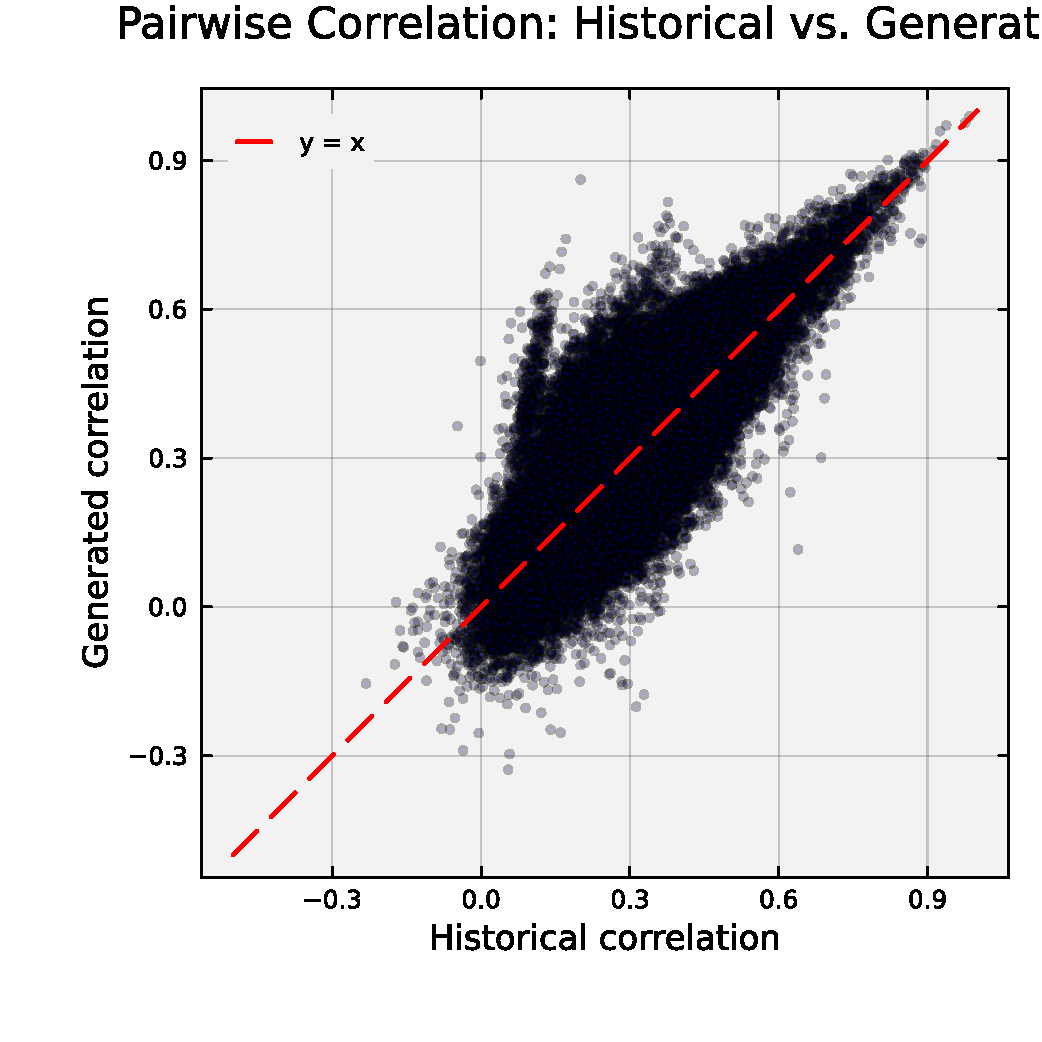
\includegraphics[width=0.45\textwidth]{figs/Fig_finance_correlation.pdf}
\caption{Pairwise correlation: historical vs.\ generated. Each point represents one of $89{,}676$ asset pairs. The scatter around $y=x$ shows partial preservation of cross-asset dependence structure (Frobenius error $26.3\%$ vs.\ $15.6\%$ for bootstrap).}
\label{fig:finance-correlation}
\end{figure}

\begin{figure}[h]
\centering
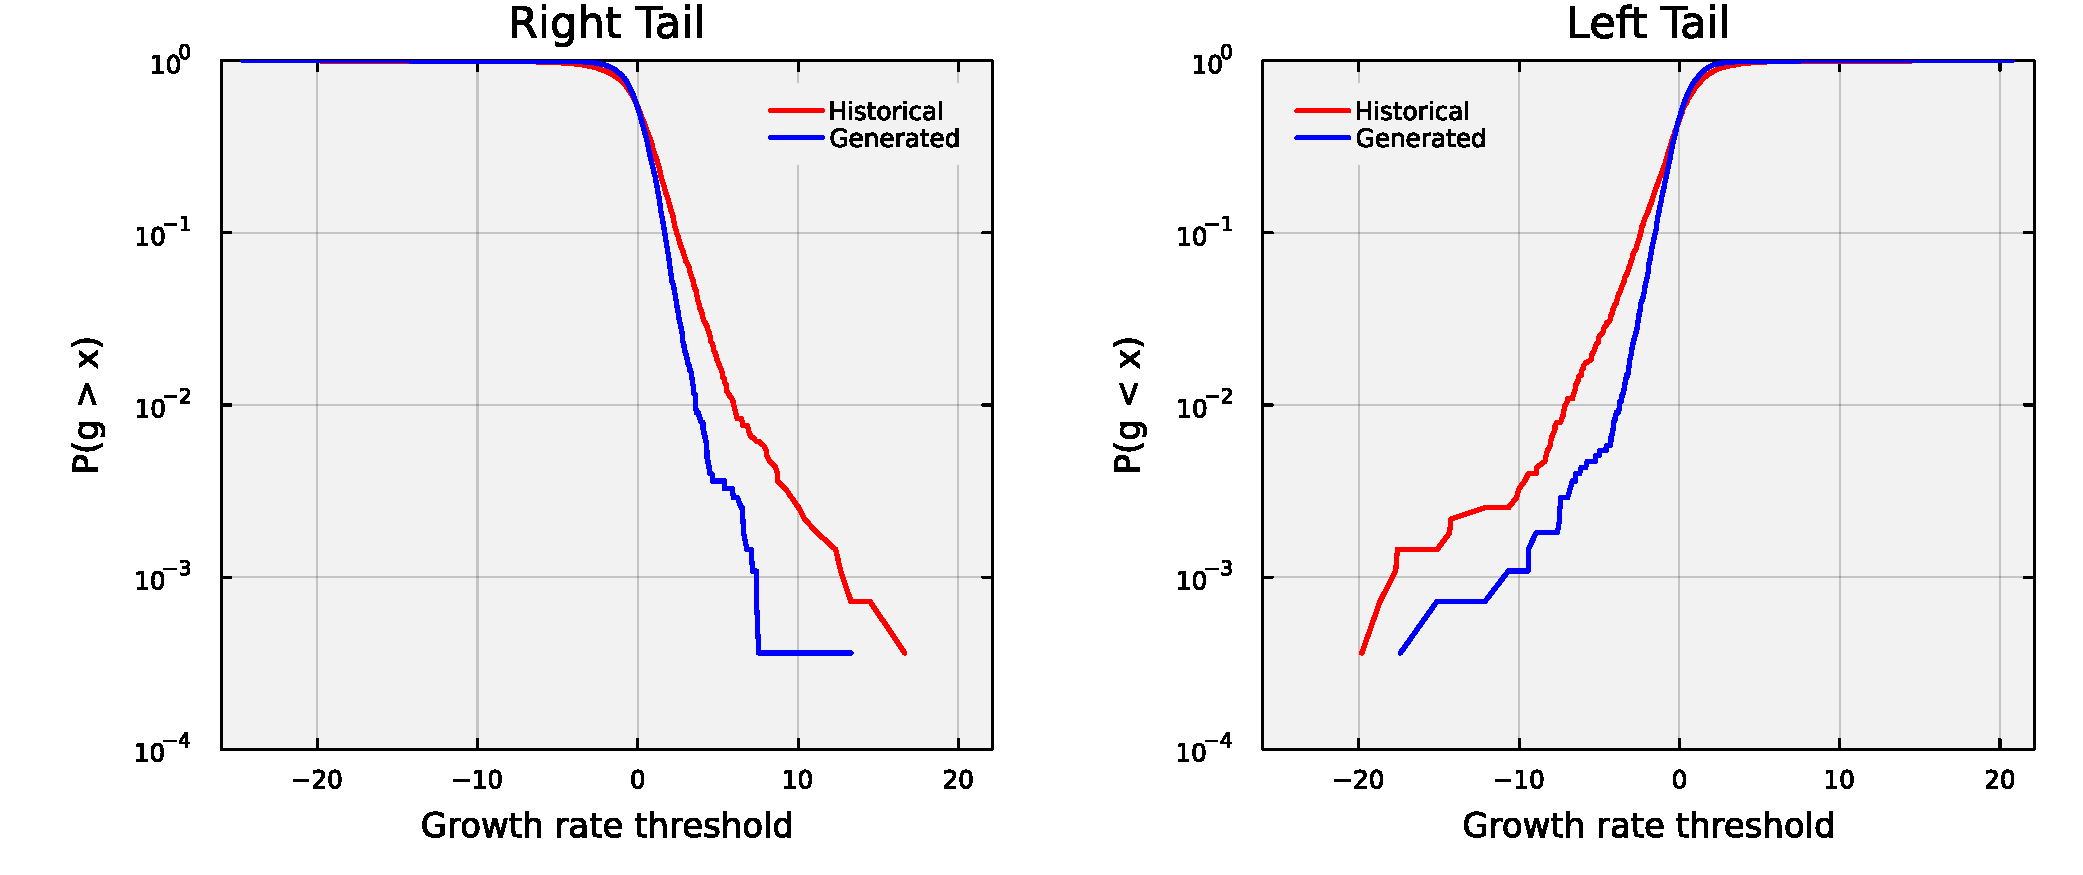
\includegraphics[width=0.75\textwidth]{figs/Fig_finance_tail_survival.pdf}
\caption{Empirical survival functions of equal-weighted portfolio returns. Both right tail $P(g > x)$ and left tail $P(g < x)$ match closely on a log scale.}
\label{fig:finance-tails}
\end{figure}

\subsection{Sequential Generation and Temporal Properties}

The i.i.d.\ pool above validates marginal fidelity but says nothing about temporal dynamics. Real equity returns exhibit two key temporal properties: (i)~returns are essentially unpredictable (near-zero autocorrelation), and (ii)~squared returns (a proxy for volatility) are highly autocorrelated and decay slowly, a phenomenon known as \emph{volatility clustering}~\cite{contStylizedFactsAsset2001}. We tested how far the stochastic attention sampler could go toward reproducing these properties.

\paragraph{Protocol.}
We generated a sequential time series of daily return vectors using the MALA sampler (Algorithm~\ref{alg:mala}) with warm-starting: each day's chain was initialized at the previous day's endpoint, creating temporal continuity in the chain trajectory.
We set $\beta = 12$ (below the main operating point $\beta{=}25$) to ensure adequate MALA mixing within $T_{\text{inner}}{=}200$ inner steps per day.
Algorithm~\ref{alg:mala-sequential} gives the pseudocode.

\begin{algorithm}[h]
\caption{MALA Warm-Start Sequential Return Generation}\label{alg:mala-sequential}
\begin{algorithmic}[1]
\REQUIRE Scaled memory matrix $\mathbf{X}\in\mathbb{R}^{d\times K}$, raw memory matrix $\mathbf{M}\in\mathbb{R}^{d\times K}$, inverse temperature $\beta$, step size $\alpha$, inner steps $T_{\text{inner}}$, number of days $T_{\text{days}}$
\ENSURE Synthetic return matrix $\hat{\mathbf{G}}\in\mathbb{R}^{T_{\text{days}}\times d}$
\STATE $k \sim \mathrm{Uniform}\{1,\dots,K\}$
\STATE $\boldsymbol{\xi} \leftarrow \mathbf{X}_{:,k} + 0.01\,\boldsymbol{\eta}, \quad \boldsymbol{\eta}\sim\mathcal{N}(\mathbf{0},\mathbf{I}_d)$ \hfill $\triangleright$ initialize near random memory
\FOR{$t = 1, 2, \dots, T_{\text{days}}$}
    \STATE Run $T_{\text{inner}}$ steps of Algorithm~\ref{alg:mala} from $\boldsymbol{\xi}$; set $\boldsymbol{\xi} \leftarrow$ endpoint \hfill $\triangleright$ warm-start
    \STATE $\hat{\mathbf{G}}_{t,:} \leftarrow \mathbf{M}\,\operatorname{softmax}(\beta\,\mathbf{X}^{\top}\boldsymbol{\xi})$ \hfill $\triangleright$ project to growth-rate space
\ENDFOR
\end{algorithmic}
\end{algorithm}

We generated $T_{\text{days}} = 2{,}766$ synthetic trading days (matching the historical sample size) with $T_{\text{inner}} = 200$, $\alpha = 0.01$, and $\beta = 12$. The mean MALA acceptance rate was 99.4\%, confirming that the ULA discretization bias is negligible at this operating point.

\paragraph{Stylized Fact~2: Near-zero return autocorrelation.}
Figure~\ref{fig:finance-acf-combined} (top row) shows the autocorrelation function of raw returns for five representative tickers. The generated ACF (blue) lay within the 99\% confidence interval for white noise at all lags $\geq 1$, matching the historical pattern (red).

\paragraph{Stylized Fact~3: Volatility clustering.}
Figure~\ref{fig:finance-acf-combined} (bottom row) shows the autocorrelation function of squared returns. The historical series (red) exhibits the characteristic slow-decaying positive autocorrelation of volatility clustering. The generated series (blue), however, shows ACF($g^2$) $\approx 0$ at all lags; the sampler did not reproduce this effect. We verified that at the main operating point ($\beta{=}25$, $T_{\text{inner}}{=}2{,}000$), ACF($g^2$) also collapses to ${\approx}0$ (mean over $424$ tickers: $0.0005$), confirming this is a property of equilibrium sampling and not an artifact of the choice of~$\beta$.

This is a fundamental limitation of equilibrium Boltzmann sampling, not a tuning failure. The stochastic attention sampler targets the stationary distribution $p_\beta \propto \exp(-\beta E)$ at fixed~$\beta$. At stationarity, the variance of each day's output is governed by the static energy landscape and the fixed temperature; there is no mechanism for the return variance to change systematically over time. Volatility clustering in real markets arises from non-stationary dynamics: regime shifts driven by exogenous shocks, feedback loops between volatility and leverage, and time-varying risk premia~\cite{contStylizedFactsAsset2001}. Reproducing these effects within the Langevin framework would require introducing explicit temporal structure, for instance a time-varying inverse temperature $\beta(t)$ that creates exogenous volatility regimes, or coupling the sampler to a latent regime-switching process. These extensions are natural directions for future work.

\paragraph{Summary.}
Table~\ref{tab:finance-summary} makes three theoretical predictions concrete. \emph{First}, the novelty--fidelity trade-off is real and quantified: SA generates regime interpolations absent from the historical record ($\mathcal{N}=0.768\pm0.001$) while bootstrap, which replays history verbatim, achieves $\mathcal{N}=0.000$; marginal fidelity runs in the opposite direction ($64.2\%$ vs.\ $99.3\%$ KS pass). \emph{Second}, the Hopfield energy captures cross-sectional dependence independently of marginals: Frobenius error $26.3\%$ is unchanged by per-ticker affine correction, confirming that the energy geometry encodes correlation structure, not scale. \emph{Third}, volatility clustering, a non-stationary phenomenon driven by regime shifts and leverage feedback~\cite{contStylizedFactsAsset2001}, is exactly what a fixed-$\beta$ equilibrium sampler cannot reproduce; the absence is a theoretical prediction confirmed by experiment, not a tuning failure.

\begin{table}[h]
\centering
\caption{Finance experiment: principled trade-offs of equilibrium Boltzmann sampling. SA and bootstrap occupy opposite ends of a novelty--fidelity spectrum: SA generates novel regime interpolations ($\mathcal{N}=0.768\pm0.001$) that bootstrap cannot produce, while bootstrap preserves marginals by construction. The Frobenius correlation error is identical before and after affine correction, confirming the energy captures dependence independently of scale. Temporal metrics apply to the sequential MALA experiment only.}
\label{tab:finance-summary}
\small
\begin{tabular}{@{}lll@{}}
\toprule
Property & SA (corrected) & Bootstrap \\
\midrule
\multicolumn{3}{@{}l@{}}{\textit{Distributional fidelity (i.i.d.\ pool, 900 samples)}} \\
KS $p$-value (mean; 64.2\% pass at $5\%$) & 0.193 & 0.622 \\
Cross-asset Frobenius error & 26.3\% & 15.6\% \\
Novelty ($1-\max_k\cos$) & $0.768\pm0.001$ & 0.000 \\
\multicolumn{3}{@{}l@{}}{\textit{Temporal properties (MALA warm-start, 2766 days)}} \\
SF2: Return unpredictability & Reproduced [ACF($g$) in 99\% CI, $\beta{=}12$] & N/A \\
SF3: Volatility clustering & Not reproduced ($\beta{=}12$) & N/A \\
\bottomrule
\end{tabular}
\end{table}

\begin{figure}[h]
\centering
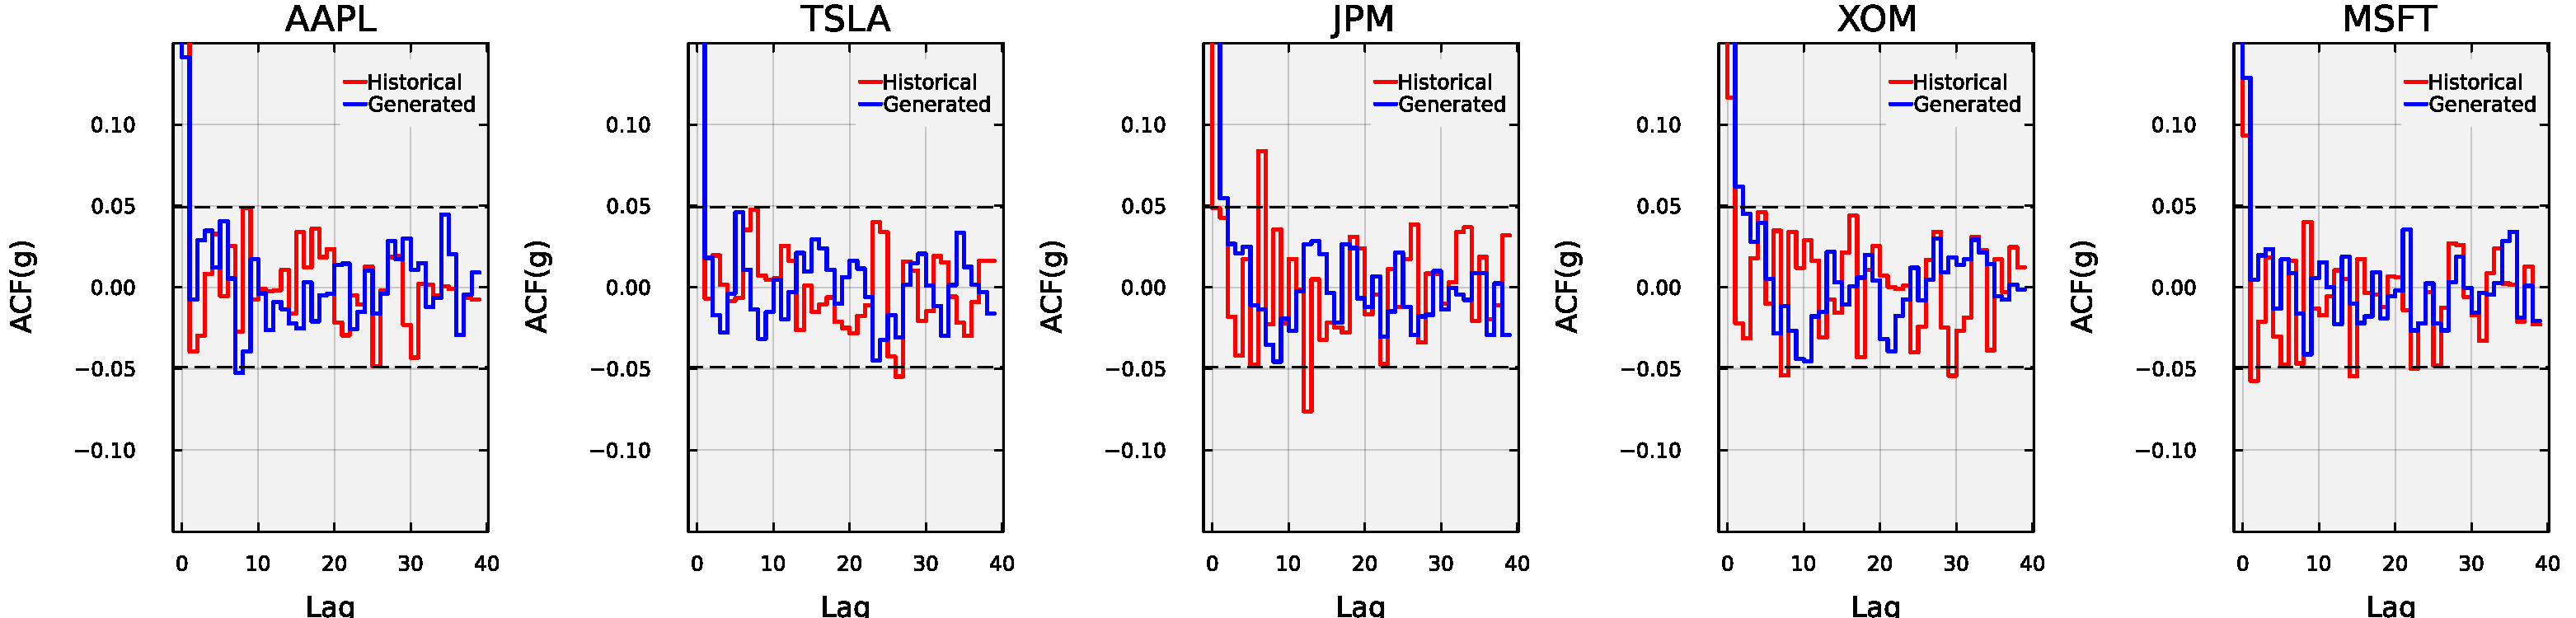
\includegraphics[width=0.95\textwidth]{figs/Fig_finance_return_acf.pdf}\\[4pt]
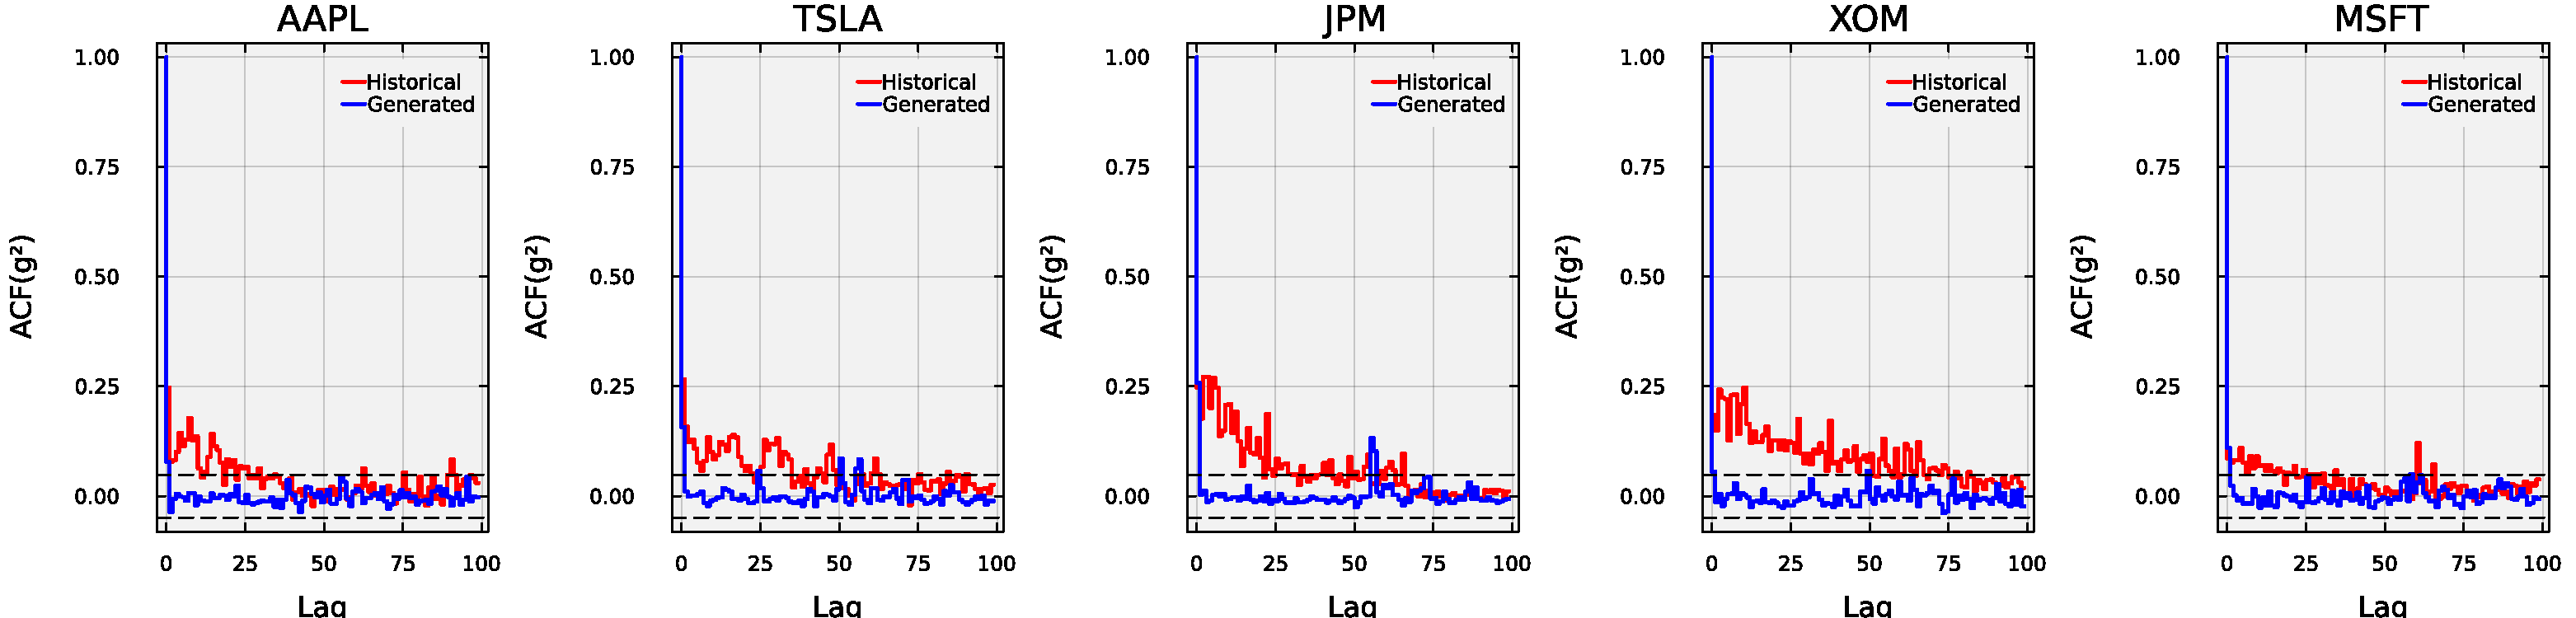
\includegraphics[width=0.95\textwidth]{figs/Fig_finance_vol_clustering.pdf}
\caption{Stylized Facts~2 and~3: Autocorrelation analysis for five S\&P~500 tickers.
\textbf{Top row}: ACF($g$): the generated series (blue) stays within the 99\% confidence band (dashed) at all lags, matching the near-zero autocorrelation of historical returns (red).
\textbf{Bottom row}: ACF($g^2$): the historical series (red) shows persistent positive autocorrelation characteristic of volatility clustering, while the generated series (blue) shows ACF($g^2$) $\approx 0$, reflecting the absence of non-stationary dynamics in the equilibrium sampler.}
\label{fig:finance-acf-combined}
\end{figure}


\section{Simpsons Character Face Generation}\label{app:simpsons}

To test whether the stochastic attention sampler generalizes from grayscale digit images to structured natural images at larger scale, we applied Algorithm~\ref{alg:stochastic-attention} to a corpus of $1{,}000$ Simpsons character face images, each downsampled to $64\times 64$ pixels and converted to grayscale, yielding pattern vectors in $\mathbb{R}^{d}$ with $d=4{,}096$, a $5.2\times$ scale-up over the MNIST experiment ($d=784$).

\paragraph{Data and setup.}
We selected $K=100$ images uniformly at random (fixed seed), matching the MNIST memory bank size to enable direct metric comparison. Each image was flattened in row-major order and normalized to unit $\ell_2$ norm to form the memory matrix $\mathbf{X}\in\mathbb{R}^{4096\times 100}$ (load ratio $K/d\approx 0.024$, well below capacity).

\paragraph{Choosing $\beta$ via the SNR rule.}
At $d=4{,}096$, the MNIST value $\beta=2{,}000$ gives $\mathrm{SNR}=\sqrt{\alpha\beta/(2d)}\approx 0.049$, half the MNIST operating point ($\mathrm{SNR}\approx 0.113$). At this lower SNR the noise overwhelms the gradient, inflating the chain norm above unity and placing samples far from the memory manifold (empirically: energy $\approx +0.53$). The SNR rule gives
\begin{equation*}
\beta = \mathrm{SNR}_{\mathrm{MNIST}}^{2}\cdot\frac{2d}{\alpha}
= 0.01276 \times \frac{2\times 4096}{0.01} \approx 10{,}449.
\end{equation*}
We used $\beta=10{,}000$ ($\mathrm{SNR}=0.110$), recovering the MNIST operating point. All other hyperparameters were identical to the MNIST experiment: $\alpha=0.01$, 30 independent chains initialized near distinct stored patterns ($\sigma_{\mathrm{init}}=0.01$), $T=5{,}000$ iterations, burn-in $2{,}000$, thin every 100 then sub-sample 5 per chain, yielding $30\times 5=150$ samples per method. The MALA acceptance rate exceeded 99\%, confirming that ULA discretization bias is negligible.

\paragraph{Temperature spectrum.}
Figure~\ref{fig:simpsons-spectrum} shows four samples at each of six inverse temperatures spanning $\beta\in\{500,1000,2000,5000,10000,20000\}$, corresponding to $\mathrm{SNR}\in\{0.025,0.035,0.049,0.078,0.110,0.156\}$. The noise-to-retrieval transition tracked SNR, not the raw $\beta$ value: rows below $\mathrm{SNR}\approx 0.05$ show diffuse gray images, while rows at $\mathrm{SNR}\geq 0.110$ yield recognizable character faces.

\begin{figure}[h]
\centering
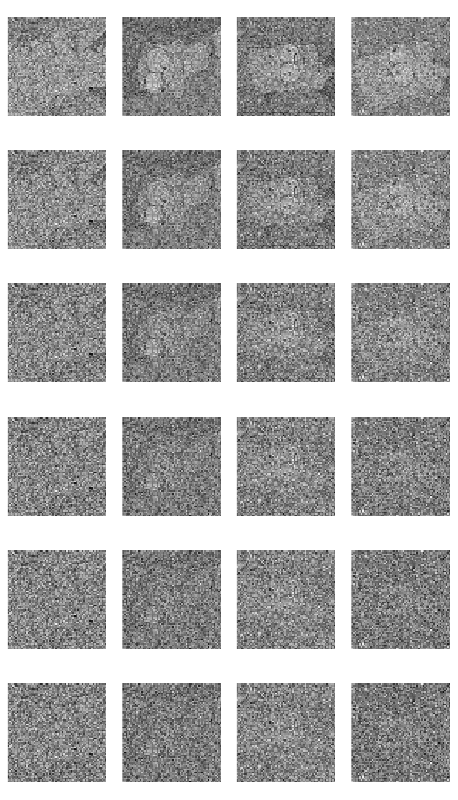
\includegraphics[width=0.65\textwidth]{figs/Fig_simpsons_beta_spectrum.png}
\caption{Temperature spectrum for Simpsons character images ($K{=}100$, $d{=}4{,}096$, $\alpha{=}0.01$). Each row shows 4 SA samples at one inverse temperature; rows are ordered from high $\beta$ (top, $\beta{=}20{,}000$, $\mathrm{SNR}{=}0.156$) to low $\beta$ (bottom, $\beta{=}500$, $\mathrm{SNR}{=}0.025$). The operating point $\beta{=}10{,}000$ ($\mathrm{SNR}{=}0.110$, row 2 from top) reproduces the MNIST SNR and yields structured character faces.}
\label{fig:simpsons-spectrum}
\end{figure}

\paragraph{Quantitative comparison.}
Table~\ref{tab:simpsons-baselines} reports metrics for all five methods at $\beta=10{,}000$. The relative ranking matches the MNIST experiment exactly: SA and MALA dominated all non-Langevin baselines on every axis simultaneously, and both Langevin methods were statistically indistinguishable. SA novelty ($0.159\pm 0.000$) was comparable to the MNIST value ($0.152\pm 0.001$); mean energy ($-0.293\pm 0.000$) confirmed that samples lay on the memory manifold. Diversity was lower than MNIST ($0.293$ vs.\ $0.600$), but this reflected the higher inter-pattern correlation of face images rather than a failure of the sampler: bootstrap diversity ($0.117$) was likewise far below the MNIST value ($0.459$), indicating that the stored patterns themselves were more concentrated in the Simpsons corpus.

\begin{table}[h]
\centering
\caption{Quantitative comparison on Simpsons character faces ($K{=}100$, $d{=}4{,}096$, $\beta{=}10{,}000$, $\mathrm{SNR}=0.110$). Same protocol as Table~\ref{tab:mnist-baselines} except GMM-PCA and VAE are omitted: at $d{=}4{,}096$ with only $K{=}100$ training patterns, both methods are degenerate (GMM covariance is rank-deficient; VAE encoder--decoder cannot generalize from 100 examples in 4,096 dimensions). MALA acceptance rate: $>99\%$. Values are mean $\pm$ SE across 30 chains. Lower diversity relative to MNIST reflects higher inter-pattern correlation of face images (bootstrap diversity $0.117$ vs.\ $0.459$ for digit~``3'').}
\label{tab:simpsons-baselines}
\small
\begin{tabular}{@{}lccc@{}}
\toprule
Method & $\mathcal{N}$ $\uparrow$ & $\bar{\mathcal{D}}$ $\uparrow$ & $\bar{E}$ $\downarrow$ \\
\midrule
Bootstrap (replay)           & $0.000 \pm 0.000$ & $0.117 \pm 0.005$ & $-0.500 \pm 0.000$ \\
Gaussian perturbation        & $0.004 \pm 0.000$ & $0.124 \pm 0.004$ & $-0.496 \pm 0.000$ \\
Random convex combination    & $0.018 \pm 0.000$ & $0.001 \pm 0.000$ & $-0.482 \pm 0.000$ \\
MALA                         & $0.157 \pm 0.000$ & $0.289 \pm 0.001$ & $-0.296 \pm 0.000$ \\
\textbf{Stochastic attention} & $\mathbf{0.159 \pm 0.000}$ & $\mathbf{0.293 \pm 0.001}$ & $\mathbf{-0.293 \pm 0.000}$ \\
\bottomrule
\end{tabular}
\end{table}

\begin{figure}[h]
\centering

\includegraphics[width=0.19\textwidth]{figs/Fig_simpsons_grid_bootstrap.png}%
\hfill

\includegraphics[width=0.19\textwidth]{figs/Fig_simpsons_grid_gaussian.png}%
\hfill
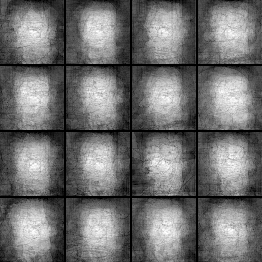
\includegraphics[width=0.19\textwidth]{figs/Fig_simpsons_grid_convex.png}%
\hfill
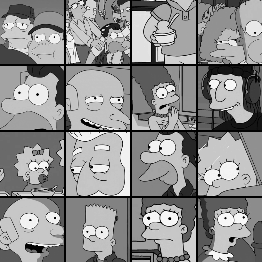
\includegraphics[width=0.19\textwidth]{figs/Fig_simpsons_grid_mala.png}%
\hfill
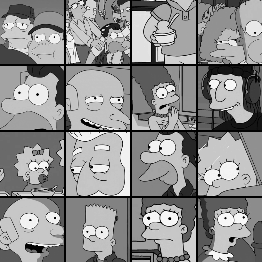
\includegraphics[width=0.19\textwidth]{figs/Fig_simpsons_grid_sa.png}

\small
\makebox[0.19\textwidth]{\centering (a) Bootstrap}%
\hfill
\makebox[0.19\textwidth]{\centering (b) Gaussian}%
\hfill
\makebox[0.19\textwidth]{\centering (c) Convex}%
\hfill
\makebox[0.19\textwidth]{\centering (d) MALA}%
\hfill
\makebox[0.19\textwidth]{\centering (e) Ours}
\caption{Generated Simpsons character face samples ($4{\times}4$ grids, $d{=}4{,}096$, $\beta{=}10{,}000$). The qualitative pattern mirrors MNIST: only the Langevin-based methods (d,\,e) produce diverse, structured face images.}
\label{fig:simpsons-grids}
\end{figure}

% ─────────────────────────────────────────────────────────────────────────────
\section{Baseline Method Specifications}\label{app:baseline-methods}
% ─────────────────────────────────────────────────────────────────────────────

This section gives complete mathematical specifications for the two learned generative
baselines in Table~\ref{tab:mnist-baselines}: GMM-PCA and the VAE.
All hyperparameters reported here were used without modification in the experiments;
the implementation is publicly available in \texttt{code/mnist-experiment/} and
\texttt{code/vae-experiment/} in the accompanying repository.

% ── GMM-PCA ──────────────────────────────────────────────────────────────────
\subsection{GMM-PCA}\label{app:gmm-pca}

\paragraph{Dimensionality reduction.}
Let $\mathbf{X}\in\mathbb{R}^{d\times K}$ be the column-normalized memory matrix
($d{=}784$, $K{=}100$). Compute the economy SVD
$\mathbf{X}=\mathbf{U}\boldsymbol{\Sigma}\mathbf{V}^{\!\top}$ and retain the top
$r{=}50$ left singular vectors, forming $\mathbf{U}_{r}\in\mathbb{R}^{d\times r}$.
Project each stored pattern to a low-dimensional code:
$\mathbf{z}_{k}=\mathbf{U}_{r}^{\!\top}\mathbf{m}_{k}\in\mathbb{R}^{r}$, $k=1,\dots,K$.
For the digit ``3'' memory matrix, the top 50 components capture $>$95\% of total variance.

\paragraph{Gaussian mixture model.}
Fit a $C{=}10$ component GMM with \emph{diagonal} covariance to the code matrix
$\mathbf{Z}{=}[\mathbf{z}_1|\cdots|\mathbf{z}_K]\in\mathbb{R}^{r\times K}$ via
Expectation-Maximization~\cite{dempsterMaximumLikelihoodIncomplete1977}:
\begin{equation}
  p(\mathbf{z}) = \sum_{c=1}^{C}\pi_c\,
  \mathcal{N}\!\bigl(\mathbf{z};\,\boldsymbol{\mu}_c,\,\mathrm{diag}(\boldsymbol{\sigma}_c^2)\bigr),
  \quad \sum_{c=1}^{C}\pi_c=1,\quad \pi_c\geq 0.
\end{equation}
Parameters $\{\pi_c,\boldsymbol{\mu}_c,\boldsymbol{\sigma}_c^2\}_{c=1}^{C}$ are estimated
by EM with K-means$\texttt{++}$ initialization and convergence tolerance $10^{-8}$ on the
log-likelihood.
The diagonal-covariance constraint prevents singularity when $K>r$ and is equivalent to
assuming conditionally independent PCA coordinates within each component.

\paragraph{Sampling.}
To draw one sample: (i) sample component $c\sim\mathrm{Categorical}(\boldsymbol{\pi})$;
(ii) sample $\tilde{\mathbf{z}}\sim\mathcal{N}(\boldsymbol{\mu}_c,\mathrm{diag}(\boldsymbol{\sigma}_c^2))$;
(iii) reconstruct $\hat{\boldsymbol{\xi}}=\mathbf{U}_{r}\tilde{\mathbf{z}}$ and
renormalize to unit $\ell_2$ norm.
The 150 evaluation samples are drawn i.i.d.\ under this procedure with a fixed seed.

\paragraph{Hyperparameters.}
$r{=}50$ PCA components; $C{=}10$ GMM components; K-means$\texttt{++}$ initialization;
EM convergence tolerance $10^{-8}$; no regularization beyond the diagonal-covariance constraint.

% ── VAE ──────────────────────────────────────────────────────────────────────
\subsection{Variational Autoencoder}\label{app:vae}

\paragraph{Architecture.}
The encoder maps $\mathbf{x}\in\mathbb{R}^{784}$ to the parameters of an approximate posterior:
\begin{align}
  \mathbf{h}_1 &= \mathrm{ReLU}(\mathbf{W}_1\mathbf{x}+\mathbf{b}_1),\quad
    \mathbf{W}_1\in\mathbb{R}^{256\times 784}, \\
  \mathbf{h}_2 &= \mathrm{ReLU}(\mathbf{W}_2\mathbf{h}_1+\mathbf{b}_2),\quad
    \mathbf{W}_2\in\mathbb{R}^{128\times 256}, \\
  \boldsymbol{\mu}_\phi(\mathbf{x}) &= \mathbf{W}_\mu\mathbf{h}_2+\mathbf{b}_\mu,\quad
    \mathbf{W}_\mu\in\mathbb{R}^{8\times 128}, \\
  \log\boldsymbol{\sigma}^2_\phi(\mathbf{x}) &= \mathbf{W}_\sigma\mathbf{h}_2+\mathbf{b}_\sigma,\quad
    \mathbf{W}_\sigma\in\mathbb{R}^{8\times 128}.
\end{align}
The decoder is architecturally symmetric: $8\to128\to256\to784$, with ReLU activations on
hidden layers and a linear output.
All weight matrices are Glorot-uniform initialized; biases are zero-initialized.
The decoder output is renormalized to unit $\ell_2$ norm before computing metrics, matching
the normalization convention of all other methods in Table~\ref{tab:mnist-baselines}.

\paragraph{Objective.}
We minimize the $\beta$-VAE objective~\cite{higginsBetaVAELearningBasic2017}:
\begin{equation}
  \mathcal{L}(\phi,\theta;\mathbf{x})
  = \underbrace{\bigl\lVert\mathbf{x}-\hat{\mathbf{x}}_\theta(\mathbf{z})\bigr\rVert_2^2}
    _{\text{reconstruction}}
  +\; \beta_{\mathrm{KL}}\underbrace{D_{\mathrm{KL}}\!\bigl(
    q_\phi(\mathbf{z}|\mathbf{x})\,\big\|\,\mathcal{N}(\mathbf{0},\mathbf{I})\bigr)}
    _{\text{regularization}},
\label{eq:vae-elbo}
\end{equation}
where $q_\phi(\mathbf{z}|\mathbf{x})=\mathcal{N}(\boldsymbol{\mu}_\phi(\mathbf{x}),
\mathrm{diag}(\boldsymbol{\sigma}^2_\phi(\mathbf{x})))$ and the reparameterization trick
$\mathbf{z}=\boldsymbol{\mu}_\phi(\mathbf{x})+\boldsymbol{\sigma}_\phi(\mathbf{x})\odot
\boldsymbol{\epsilon}$, $\boldsymbol{\epsilon}\sim\mathcal{N}(\mathbf{0},\mathbf{I})$,
enables gradient flow through the sampling step.
The KL term has a closed form:
\begin{equation}
  D_{\mathrm{KL}} = \tfrac{1}{2}\sum_{j=1}^{8}\bigl[
    \mu_{\phi,j}^2+\sigma_{\phi,j}^2 - \log\sigma_{\phi,j}^2 - 1\bigr].
\end{equation}

\paragraph{Two-phase training protocol.}
Training directly with the full $\beta$-VAE objective on a small dataset ($K{=}100$)
causes \emph{posterior collapse}: the encoder ignores the input, the KL term drives every
latent dimension to $\mathcal{N}(0,1)$, and the decoder learns a constant map.
We prevent this with a two-phase schedule:
\begin{enumerate}
  \item \textbf{Warm-up (epochs 1--2{,}000):} Train with $\beta_{\mathrm{KL}}{=}0$
    (reconstruction-only autoencoder objective). This establishes a non-degenerate
    encoder (one that uses the latent code productively) before any regularization pressure
    is applied.
  \item \textbf{Fine-tuning (epochs 2{,}001--4{,}000):} Introduce the KL term with
    $\beta_{\mathrm{KL}}{=}0.0001$ and a linear warmup schedule
    ($\beta_{\mathrm{KL}}(t) = 0.0001\cdot(t/2000)$ for $t\in[1,2000]$).
    The small final weight provides light regularization toward the Gaussian prior without
    overriding the reconstruction signal.
\end{enumerate}
The warm-up phase is equivalent to a hard $\beta$-annealing schedule and is standard practice
for low-data VAE training~\cite{lucasHowAvoidTrivial2019}.
On large datasets ($K\gg10^4$), the reconstruction gradient swamps the KL term and posterior
collapse does not occur; the two-phase protocol is needed here specifically because
$K{=}100$ makes the per-sample gradients noisy relative to the KL regularization pressure.

\paragraph{Optimization and sampling.}
Optimizer: Adam~\cite{kingmaAdamMethodStochastic2014} with learning rate $10^{-3}$,
$\beta_1{=}0.9$, $\beta_2{=}0.999$, $\varepsilon{=}10^{-8}$, batch size $K{=}100$
(full-dataset batches throughout).
No weight decay, dropout, or data augmentation was applied.
At evaluation time, 150 samples are drawn by sampling
$\mathbf{z}\sim\mathcal{N}(\mathbf{0},\mathbf{I}_8)$ and decoding
$\hat{\mathbf{x}}=\hat{\mathbf{x}}_\theta(\mathbf{z})$, then renormalizing to unit norm.

\paragraph{Hyperparameter selection.}
The final configuration (latent dim 8, $\beta_{\mathrm{KL}}{=}0.0001$) was chosen by a
grid search over latent dimension $\in\{4,8,16,32\}$ and $\beta_{\mathrm{KL}}\in\{0.1,0.01,0.001,0.0001\}$,
evaluating novelty and diversity on the held-out generation protocol.
Latent dim 8 with $\beta_{\mathrm{KL}}{=}0.0001$ achieved $\mathcal{N}{=}0.214\pm0.005$,
$\bar{\mathcal{D}}{=}0.441\pm0.008$, outperforming all other static baselines including
GMM-PCA ($\mathcal{N}{=}0.198$, $\bar{\mathcal{D}}{=}0.419$).
Smaller latent dimensions or larger $\beta_{\mathrm{KL}}$ values degraded novelty and
diversity, while larger latent dimensions showed posterior collapse symptoms
(diversity collapsing to $\bar{\mathcal{D}}{<}0.05$ at latent dim 32 with $\beta_{\mathrm{KL}}{=}0.01$).

% ── DDPM ────────────────────────────────────────────────────────────────────
\subsection{Denoising Diffusion Probabilistic Model (DDPM)}\label{app:ddpm}

We implement a standard DDPM~\cite{hoDenoisingDiffusionProbabilistic2020} operating on the
same flattened, unit-norm MNIST vectors used by all other methods.

\paragraph{Architecture.}
Since the data are flattened 784-dimensional vectors (not 2D images), we use an MLP denoiser
rather than a convolutional U-Net. The input at each timestep~$t$ is the concatenation of the
noisy vector $\mathbf{x}_t\in\mathbb{R}^{784}$ and a sinusoidal timestep embedding
$\mathbf{e}_t\in\mathbb{R}^{64}$, giving an 848-dimensional input. The network is
$848\to512~(\mathrm{ReLU})\to256~(\mathrm{ReLU})\to512~(\mathrm{ReLU})\to784$,
predicting the noise $\boldsymbol{\epsilon}$.

\paragraph{Diffusion schedule.}
We use $T{=}200$ diffusion steps with a linear variance schedule
$\beta_1{=}10^{-4},\;\beta_T{=}0.02$, following Ho et al.~\cite{hoDenoisingDiffusionProbabilistic2020}.
The forward process is $q(\mathbf{x}_t|\mathbf{x}_0)=\mathcal{N}(\sqrt{\bar\alpha_t}\,\mathbf{x}_0,\;(1{-}\bar\alpha_t)\mathbf{I})$
where $\bar\alpha_t=\prod_{s=1}^{t}(1-\beta_s)$.

\paragraph{Training.}
We train for $5{,}000$ epochs using Adam~\cite{kingmaAdamMethodStochastic2014}
(learning rate $10^{-3}$) with full-batch updates ($K{=}100$).
At each epoch, we sample random timesteps $t\sim\mathrm{Uniform}\{1,\dots,T\}$ for each training
image, draw noise $\boldsymbol{\epsilon}\sim\mathcal{N}(\mathbf{0},\mathbf{I})$, compute
$\mathbf{x}_t=\sqrt{\bar\alpha_t}\,\mathbf{x}_0+\sqrt{1{-}\bar\alpha_t}\,\boldsymbol{\epsilon}$,
and minimize the MSE loss $\lVert\boldsymbol{\epsilon}-\hat{\boldsymbol{\epsilon}}_\theta(\mathbf{x}_t,t)\rVert_2^2$.

\paragraph{Sampling.}
We generate 150 samples via the standard reverse process starting from
$\mathbf{x}_T\sim\mathcal{N}(\mathbf{0},\mathbf{I})$ and iterating
$\mathbf{x}_{t-1}=\frac{1}{\sqrt{\alpha_t}}\bigl(\mathbf{x}_t-\frac{\beta_t}{\sqrt{1-\bar\alpha_t}}\hat{\boldsymbol{\epsilon}}_\theta(\mathbf{x}_t,t)\bigr)+\sqrt{\beta_t}\,\mathbf{z}$
for $t=T,\dots,1$. Each output is $\ell_2$-normalized to match the convention of all other methods.

\paragraph{Result.}
The DDPM produced samples with $\mathcal{N}{=}0.938$, $\bar{\mathcal{D}}{=}0.991$, and
max-cosine similarity to the nearest stored pattern of $0.062$, indistinguishable from
isotropic Gaussian noise ($0.057$; Appendix~\ref{app:noise-control}).
The training loss plateaued at ${\approx}0.855$ (close to the expected MSE for predicting
random noise), indicating that the denoiser failed to learn the data distribution.
This is the expected behavior: DDPM requires thousands to millions of training images to
estimate a score function across $T{=}200$ noise levels; with only $K{=}100$ images in
$\mathbb{R}^{784}$, the model is severely underspecified.
Stochastic attention avoids this failure mode entirely because its score function is available
in closed form from the Hopfield energy, requiring no training data beyond the stored patterns
themselves.

% ─────────────────────────────────────────────────────────────────────────────
\section{Step-Size Sweep: ULA vs.\ MALA}\label{app:stepsize-sweep}
% ─────────────────────────────────────────────────────────────────────────────

At the operating point used throughout this paper ($\alpha{=}0.01$, $\beta{=}2000$), MALA acceptance exceeds $99\%$ and the two algorithms are trivially equivalent. A natural question is: \emph{at what step size does the ULA discretization bias become significant, and how does sample quality degrade?} We swept $\alpha\in\{0.001,0.005,0.01,0.02,0.05,0.1,0.2,0.3,0.5\}$ on MNIST digit~``3'' ($K{=}100$, $d{=}784$, $\beta{=}2000$), running 30 chains per method with the same protocol as the main MNIST experiment (Table~\ref{tab:mnist-baselines}).

Table~\ref{tab:stepsize-sweep} and Figure~\ref{fig:stepsize-sweep} reveal three regimes:
\begin{enumerate}
  \item \textbf{Equivalent regime} ($\alpha\leq 0.02$): MALA acceptance $>97\%$; ULA and MALA metrics are indistinguishable ($\Delta E < 0.003$).
  \item \textbf{Divergence regime} ($\alpha\in[0.05,0.1]$): acceptance drops to $75$--$91\%$; ULA bias becomes detectable but small ($\Delta\mathcal{N}\approx 0.007$, $\Delta E \approx 0.011$).
  \item \textbf{MALA-frozen regime} ($\alpha\geq 0.2$): MALA acceptance collapses to $0\%$ (the chain freezes at its initialization) while ULA continues to produce samples with gracefully degrading quality (rising energy, increasing novelty as the noise term dominates).
\end{enumerate}
The practical divergence threshold is $\alpha\approx 0.1$ ($75\%$ acceptance, $\Delta E = 0.011$). At the paper's operating point ($\alpha{=}0.01$), ULA bias is negligible ($\Delta E = 0.0018$). At large step sizes, ULA is \emph{preferable} to MALA: MALA freezes entirely because the large Langevin proposals are almost always rejected, while ULA, which unconditionally accepts every proposal, continues to explore the energy landscape.

\begin{table}[h]
\centering
\caption{Step-size sweep on MNIST digit ``3'' ($K{=}100$, $d{=}784$, $\beta{=}2000$). ULA and MALA are indistinguishable for $\alpha\leq 0.02$. At $\alpha\geq 0.2$, MALA acceptance collapses and the chain freezes, while ULA continues sampling.}
\label{tab:stepsize-sweep}
\small
\begin{tabular}{@{}rcccccc@{}}
\toprule
$\alpha$ & Accept & \multicolumn{2}{c}{Novelty} & \multicolumn{2}{c}{Diversity} & $\Delta E$ \\
 & rate & ULA & MALA & ULA & MALA & (ULA$-$MALA) \\
\midrule
0.001 & $>$0.99 & 0.151 & 0.150 & 0.595 & 0.595 & $<$0.001 \\
0.005 & $>$0.99 & 0.151 & 0.151 & 0.599 & 0.597 & $<$0.001 \\
0.01  & 0.992 & 0.152 & 0.151 & 0.600 & 0.598 & 0.002 \\
0.02  & 0.978 & 0.153 & 0.151 & 0.600 & 0.598 & 0.003 \\
0.05  & 0.911 & 0.155 & 0.151 & 0.602 & 0.598 & 0.006 \\
0.1   & 0.747 & 0.158 & 0.151 & 0.605 & 0.597 & 0.011 \\
0.2   & 0.000 & 0.165 & 0.000 & 0.612 & 0.000 & --- \\
0.3   & 0.000 & 0.172 & 0.000 & 0.619 & 0.000 & --- \\
0.5   & 0.000 & 0.189 & 0.000 & 0.635 & 0.000 & --- \\
\bottomrule
\end{tabular}
\end{table}

\begin{figure}[h]
\centering
\IfFileExists{figs/Fig_stepsize_sweep_ula_vs_mala.pdf}{%
  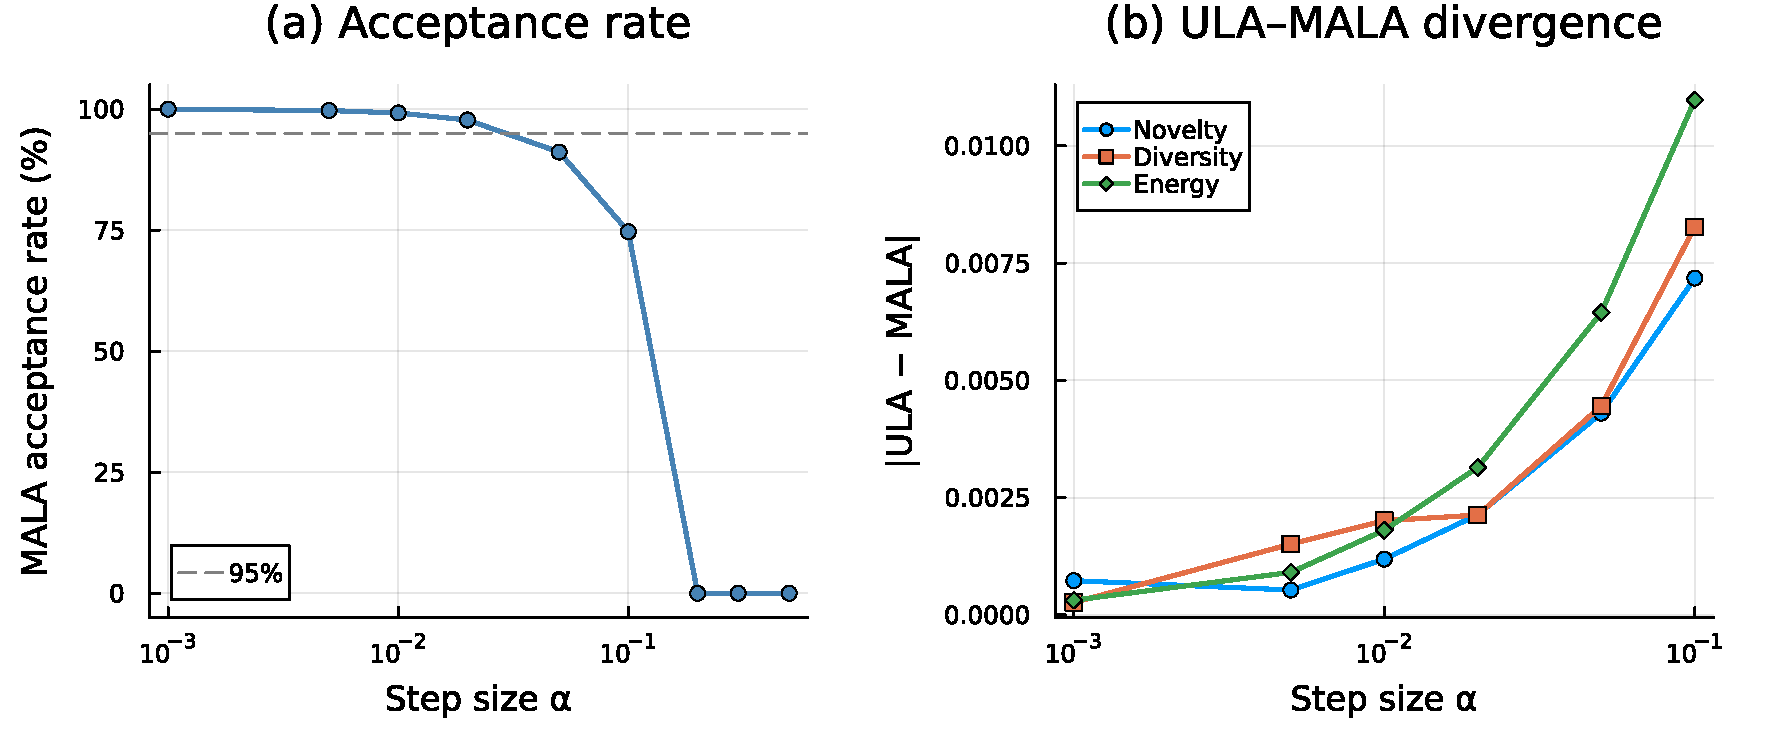
\includegraphics[width=0.95\textwidth]{figs/Fig_stepsize_sweep_ula_vs_mala.pdf}%
}{%
  \framebox[0.95\textwidth]{\rule{0pt}{4cm}\texttt{[Figure will be generated by run\_stepsize\_sweep.jl]}}%
}
\caption{Step-size sweep: ULA vs.\ MALA on MNIST digit ``3'' ($\beta{=}2000$). \textbf{(a)}~MALA acceptance rate vs.\ step size $\alpha$. Acceptance exceeds $95\%$ for $\alpha\leq 0.02$ and collapses to $0\%$ at $\alpha\geq 0.2$. \textbf{(b)}~Absolute difference between ULA and MALA metrics. All three metrics (novelty, diversity, energy) diverge smoothly as $\alpha$ increases through the $[0.05,0.1]$ band.}
\label{fig:stepsize-sweep}
\end{figure}

% ─────────────────────────────────────────────────────────────────────────────
\section{Gaussian Noise Control at $\beta{=}200$}\label{app:noise-control}
% ─────────────────────────────────────────────────────────────────────────────

At $\beta{=}200$ (SNR$=0.036$, the generation regime), SA achieves high novelty ($0.547$) and diversity ($0.885$) but the mean Hopfield energy is positive ($+1.47$), meaning samples lie outside the attractor manifold. A natural concern is that these metrics could be achieved trivially by high-temperature noise that bears no structural relationship to the stored patterns. We test this by comparing SA against two Gaussian noise controls on MNIST digit~``3'' ($K{=}100$, $d{=}784$).

\paragraph{Controls.}
\emph{Matched Gaussian}: for each pixel $j$, we estimate the mean $\mu_j$ and variance $\sigma_j^2$ of the 150 SA samples and draw i.i.d.\ $\mathcal{N}(\mu_j, \sigma_j^2)$; this is the strongest possible Gaussian that matches SA's marginal pixel statistics. \emph{Isotropic Gaussian}: we draw $\mathbf{g}\sim\mathcal{N}(\mathbf{0},\mathbf{I}_d)$ and rescale to match the mean norm of SA samples ($\lVert\boldsymbol{\xi}\rVert\approx 2.22$). Both controls produce 150 samples.

\paragraph{Results.}
Table~\ref{tab:noise-control} and Figure~\ref{fig:noise-control} present the comparison. The key separating metric is \emph{maximum cosine similarity} to the nearest stored pattern (Max-$\cos$): SA retains $0.453$, meaning each sample sits roughly halfway between the stored-pattern manifold ($1.0$) and random directions (${\approx}0.06$ in $\mathbb{R}^{784}$). The matched Gaussian achieves only $0.328$ despite sharing SA's per-pixel moments, and isotropic noise achieves $0.057$ (the random-direction baseline). Hopfield energy separates the methods in the same order: SA ($1.47$) $<$ matched Gaussian ($1.78$) $<$ isotropic ($2.34$).

Novelty and diversity, by contrast, are similar between SA and the matched Gaussian ($0.547$ vs.\ $0.672$ and $0.885$ vs.\ $0.878$), confirming the reviewer's observation that these metrics alone do not distinguish structured generation from noise. However, the max-cosine and energy metrics do: SA samples are geometrically closer to stored patterns because the Langevin dynamics is guided by the Hopfield energy gradient, which biases the chain toward the memory manifold even at high temperature. Gaussian noise, lacking this gradient signal, cannot achieve the same structural similarity.

Visually (Figure~\ref{fig:noise-control}), SA samples show faint but recognizable digit-3 structure (curved strokes, characteristic topology), while both Gaussian controls produce uniform static with no discernible spatial structure.

We note honestly that $\beta{=}200$ is a high-temperature regime where sample quality is limited: the noise term $\sqrt{2\alpha/\beta}\,\boldsymbol{\epsilon}$ has standard deviation $0.01$ per component, comparable to the gradient step. The samples are ``blurry-but-recognizable'' rather than crisp. Higher-fidelity generation requires operating closer to the transition band ($\beta{\approx}500$--$1000$), trading novelty for structural quality.

\begin{table}[h]
\centering
\caption{Gaussian noise control on MNIST digit ``3'' at $\beta{=}200$ (generation regime). Max-$\cos$ and energy cleanly separate SA from both Gaussian controls: SA samples retain structural similarity to stored patterns that noise cannot replicate. FD$_{\text{diag}}$ is the diagonal pixel-space Fr\'{e}chet distance to stored patterns.}
\label{tab:noise-control}
\small
\begin{tabular}{@{}lccccc@{}}
\toprule
Method & $\mathcal{N}$ $\uparrow$ & $\bar{\mathcal{D}}$ $\uparrow$ & $\bar{E}$ $\downarrow$ & Max-$\cos$ $\uparrow$ & FD$_{\text{diag}}$ $\downarrow$ \\
\midrule
Stored patterns                   & 0.000 & 0.459 & $-0.50$ & 1.000 & ---  \\
\textbf{SA ($\beta{=}200$)}       & 0.547 & 0.885 & $+1.47$ & 0.453 & 2.81 \\
Gaussian (matched $\mu,\sigma^2$) & 0.672 & 0.878 & $+1.78$ & 0.328 & 2.86 \\
Gaussian (isotropic)              & 0.943 & 1.000 & $+2.34$ & 0.057 & 3.91 \\
\bottomrule
\end{tabular}
\end{table}

\begin{figure}[h]
\centering
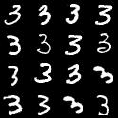
\includegraphics[width=0.19\textwidth]{figs/Fig_noise_control_stored.png}%
\hfill
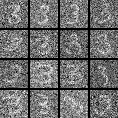
\includegraphics[width=0.19\textwidth]{figs/Fig_noise_control_sa_beta200.png}%
\hfill
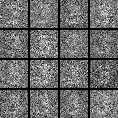
\includegraphics[width=0.19\textwidth]{figs/Fig_noise_control_gauss_matched.png}%
\hfill
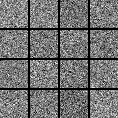
\includegraphics[width=0.19\textwidth]{figs/Fig_noise_control_gauss_iso.png}%
\hfill
\IfFileExists{figs/Fig_noise_control_maxcos_hist.pdf}{%
  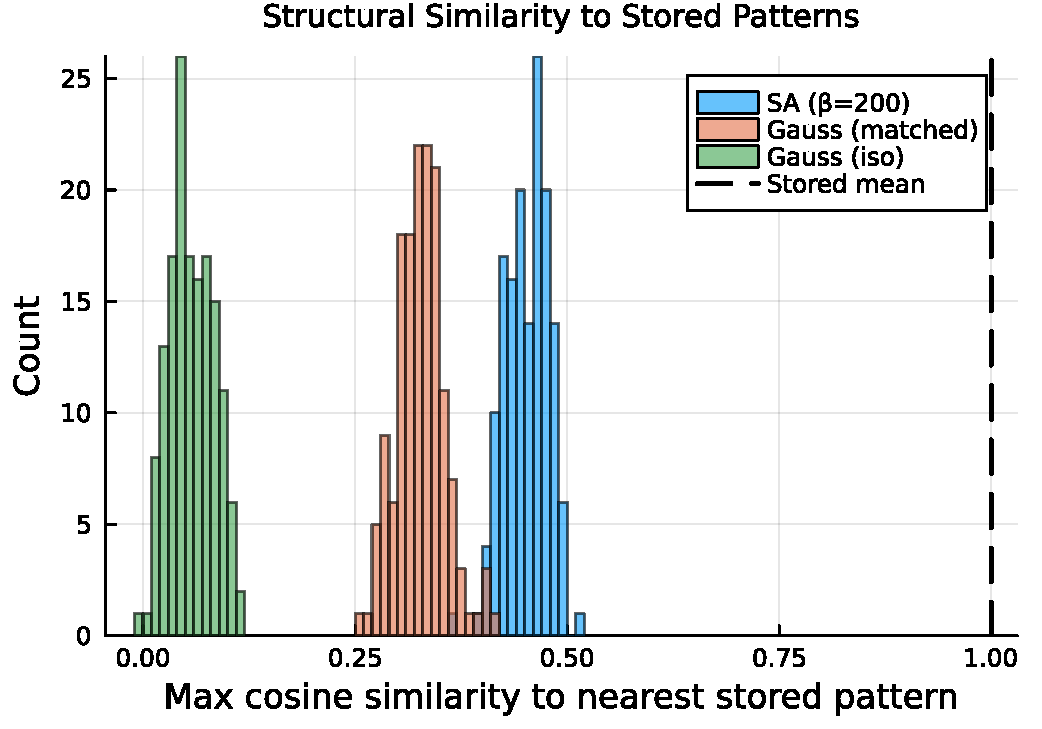
\includegraphics[width=0.19\textwidth]{figs/Fig_noise_control_maxcos_hist.pdf}%
}{%
  \framebox[0.19\textwidth]{\rule{0pt}{3cm}\small hist}%
}

\small
\makebox[0.19\textwidth]{\centering (a) Stored}%
\hfill
\makebox[0.19\textwidth]{\centering (b) SA ($\beta{=}200$)}%
\hfill
\makebox[0.19\textwidth]{\centering (c) Gauss (matched)}%
\hfill
\makebox[0.19\textwidth]{\centering (d) Gauss (iso)}%
\hfill
\makebox[0.19\textwidth]{\centering (e) Max-$\cos$ dist.}
\caption{Gaussian noise control. \textbf{(a)}~Stored digit ``3'' patterns. \textbf{(b)}~SA at $\beta{=}200$: noisy but spatially structured (curved strokes visible). \textbf{(c)}~Matched Gaussian (same per-pixel $\mu$ and $\sigma^2$ as SA): uniform static, no digit structure. \textbf{(d)}~Isotropic Gaussian (matched norm): pure noise. \textbf{(e)}~Distribution of max cosine similarity to nearest stored pattern: SA (blue) is clearly shifted right of both Gaussian controls, confirming that the Hopfield energy gradient preserves structural similarity that noise cannot replicate.}
\label{fig:noise-control}
\end{figure}

% ─────────────────────────────────────────────────────────────────────────────
\section{Scaling Experiment: SA vs.\ DDPM}\label{app:scaling}
% ─────────────────────────────────────────────────────────────────────────────

The $K{=}100$ MNIST experiment (Table~\ref{tab:mnist-baselines}) showed that DDPM fails entirely when training data are scarce, but this comparison is arguably unfair to DDPM: diffusion models are designed for large-data regimes. We therefore ran a scaling study at $K\in\{100,\,500,\,1{,}000,\,2{,}000,\,3{,}500\}$ digit-3 images (the maximum available in MNIST) to test whether DDPM catches up as $K$ grows and to characterize how SA behaves under a principled, data-dependent $\beta$ selection.

\paragraph{$\beta$ selection via entropy inflection.}
At each~$K$, we set $\beta$ using the entropy inflection criterion of Proposition~\ref{prop:entropy-derivative}: we sweep $\beta$ over a grid, compute the attention entropy $H(\beta)=-\sum_k p_k\log p_k$ where $\mathbf{p}=\mathrm{softmax}(\beta\mathbf{X}^\top\boldsymbol{\xi})$ averaged over a probe set, and identify $\beta^*$ at the inflection point (maximum $|dH/d\beta|$). This gives a principled, data-dependent operating point for each $K$ without manual tuning. For each $K$ we also report SA at $5\beta^*$ (the retrieval regime) to illustrate the temperature knob.

\paragraph{DDPM configuration.}
We use the same MLP architecture (Appendix~\ref{app:ddpm}) with $T{=}200$ diffusion steps at every~$K$. Training epochs are scaled inversely with $K$ to keep total gradient steps comparable: $5{,}000$ epochs at $K{=}100$ down to $1{,}000$ epochs at $K{=}3{,}500$.

\paragraph{Results.}
Table~\ref{tab:scaling} and Figure~\ref{fig:scaling} present the results. The key metric is max-cosine similarity to the nearest stored pattern, which distinguishes structured generation from noise.

\begin{table}[h]
\centering
\caption{Scaling experiment on MNIST digit ``3''. $\beta^*$ is set via entropy inflection at each $K$. SA operates at $\beta^*$ (generation) and $5\beta^*$ (retrieval). Max-$\cos$ measures structural similarity to stored patterns (isotropic noise baseline: ${\approx}0.06$).}
\label{tab:scaling}
\small
\begin{tabular}{@{}rrccccccccc@{}}
\toprule
$K$ & $K/d$ & $\beta^*$ & \multicolumn{3}{c}{SA (generation, $\beta{=}\beta^*$)} & \multicolumn{3}{c}{SA (retrieval, $\beta{=}5\beta^*$)} & \multicolumn{2}{c}{DDPM ($T{=}200$)} \\
\cmidrule(lr){4-6}\cmidrule(lr){7-9}\cmidrule(lr){10-11}
 & & & $\mathcal{N}$ & $\bar{\mathcal{D}}$ & max-$\cos$ & $\mathcal{N}$ & $\bar{\mathcal{D}}$ & max-$\cos$ & max-$\cos$ & train (s) \\
\midrule
100  & 0.13 & 9   & 0.874 & 0.993 & 0.126 & 0.763 & 0.969 & 0.237 & 0.061 & 34 \\
500  & 0.64 & 13  & 0.851 & 0.991 & 0.149 & 0.722 & 0.955 & 0.278 & 0.073 & 37 \\
1000 & 1.28 & 15  & 0.839 & 0.989 & 0.161 & 0.697 & 0.949 & 0.303 & 0.078 & 46 \\
2000 & 2.55 & 18  & 0.827 & 0.987 & 0.173 & 0.673 & 0.940 & 0.327 & 0.086 & 66 \\
3500 & 4.46 & 18  & 0.825 & 0.987 & 0.175 & 0.673 & 0.944 & 0.327 & 0.090 & 75 \\
\bottomrule
\end{tabular}
\end{table}

\begin{figure}[h]
\centering
\IfFileExists{figs/Fig_scaling_sa_vs_ddpm.pdf}{%
  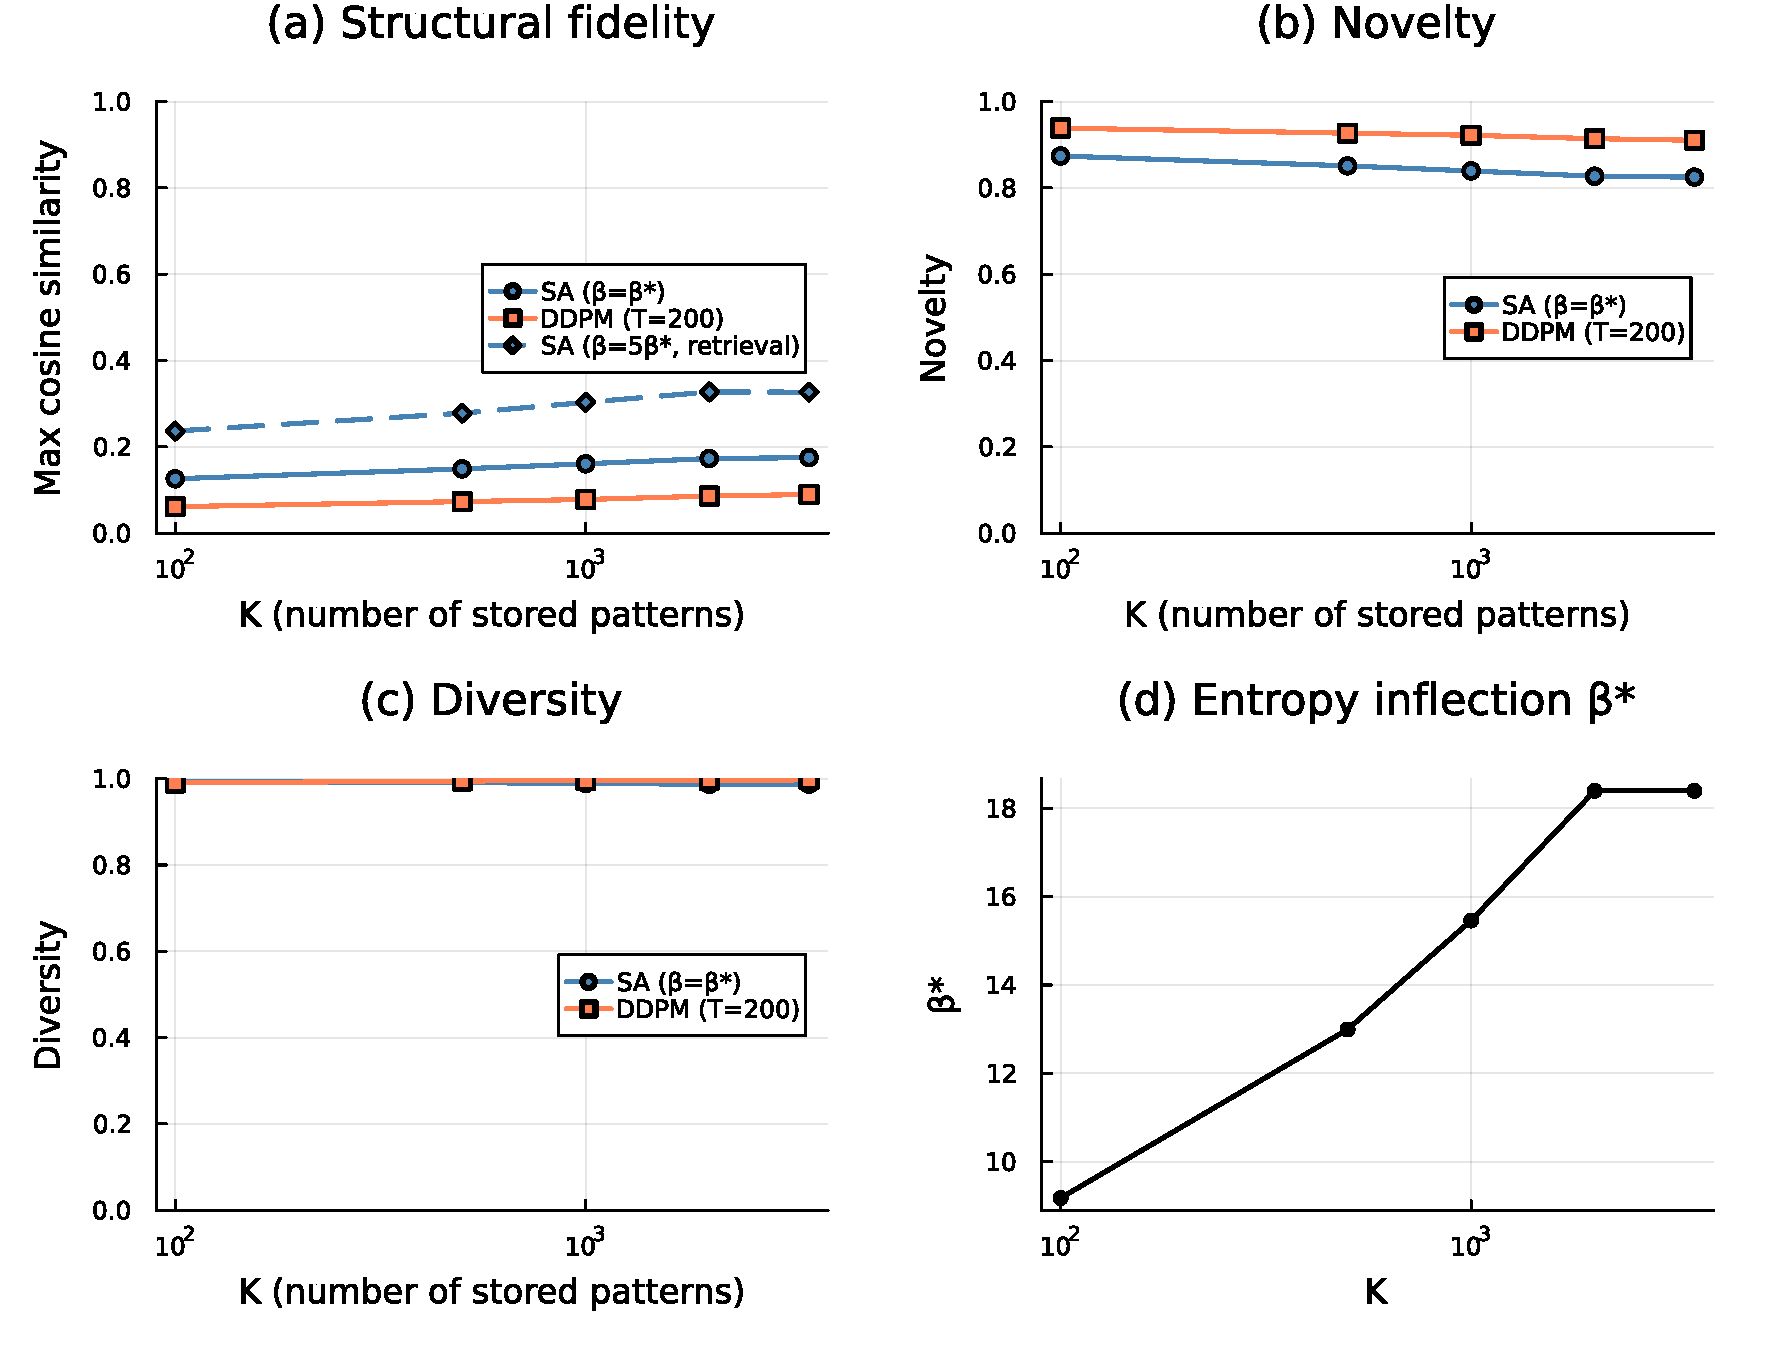
\includegraphics[width=0.95\textwidth]{figs/Fig_scaling_sa_vs_ddpm.pdf}%
}{%
  \framebox[0.95\textwidth]{\rule{0pt}{4cm}\texttt{[Figure will be generated by run\_scaling\_experiment.jl]}}%
}
\caption{Scaling experiment: SA vs.\ DDPM on MNIST digit ``3'' as the number of stored patterns $K$ increases from 100 to 3{,}500. \textbf{(a)}~Max-cosine similarity: SA at both $\beta^*$ (generation) and $5\beta^*$ (retrieval) produces samples with meaningful structural similarity to stored patterns that increases with $K$; DDPM remains near the isotropic noise floor (${\approx}0.06$) at all $K$ tested. \textbf{(b)}~Novelty. \textbf{(c)}~Diversity. \textbf{(d)}~Entropy-inflection $\beta^*$ as a function of $K$.}
\label{fig:scaling}
\end{figure}

Three findings emerge. First, DDPM's max-cosine similarity never exceeds $0.09$ across the entire range $K\in[100,\,3{,}500]$, remaining close to the isotropic noise baseline of ${\approx}0.06$. The MLP denoiser cannot learn the data distribution even with $3{,}500$ training images in $\mathbb{R}^{784}$. Second, SA's max-cosine similarity grows monotonically with $K$: from $0.126$ at $K{=}100$ to $0.175$ at $K{=}3{,}500$ in the generation regime, and from $0.237$ to $0.327$ in the retrieval regime. More stored patterns provide denser coverage of the data manifold, enabling SA to generate samples that are structurally closer to the training distribution. Third, the entropy-inflection $\beta^*$ increases with $K$ (from $9$ to $18$), consistent with the theoretical prediction that the transition temperature shifts as memory load grows. SA requires no retuning: the entropy inflection provides a principled, automatic $\beta$ at each $K$.

We acknowledge that a convolutional U-Net DDPM operating on 2D images (rather than flattened vectors) would likely perform better, particularly at larger $K$. The comparison here is deliberately controlled: both methods operate on the same flattened, unit-norm representation. The point is not that SA is universally superior to diffusion models, but that SA's training-free score function provides a structural advantage in the low-data regime ($K\lesssim 10^3$) and that this advantage persists as $K$ grows within the range tested.

\section{MALA at Generation Temperature}\label{app:mala-generation}
% ─────────────────────────────────────────────────────────────────────────────

To confirm that the ULA discretization bias is negligible in the generation regime (not just the retrieval regime), we ran the full MALA comparison at $\beta\in\{200,\,500,\,1000\}$ with the same 30-chain protocol on MNIST digit ``3'' ($K{=}100$).

\begin{table}[h]
\centering
\caption{ULA (SA) vs.\ MALA across the generation-to-retrieval spectrum. $\Delta$ columns report SA$-$MALA. All differences are negligible ($|\Delta|<0.02$), confirming that ULA bias does not affect any experimental conclusion.}
\label{tab:mala-generation}
\small
\begin{tabular}{@{}rccccccc@{}}
\toprule
$\beta$ & Accept & $\mathcal{N}_{\text{SA}}$ & $\Delta\mathcal{N}$ & $\bar{\mathcal{D}}_{\text{SA}}$ & $\Delta\bar{\mathcal{D}}$ & $\bar{E}_{\text{SA}}$ & $\Delta\bar{E}$ \\
\midrule
200  & 99.2\% & 0.548 & $+0.002$ & 0.885 & $+0.002$ & $+1.467$ & $+0.018$ \\
500  & 99.2\% & 0.375 & $+0.002$ & 0.782 & $+0.002$ & $+0.287$ & $+0.007$ \\
1000 & 99.2\% & 0.251 & $+0.002$ & 0.687 & $+0.002$ & $-0.107$ & $+0.004$ \\
\bottomrule
\end{tabular}
\end{table}

At $\beta{=}200$ (the generation regime), the deltas are: $\Delta\mathcal{N}{=}+0.002$, $\Delta\bar{\mathcal{D}}{=}+0.002$, $\Delta\bar{E}{=}+0.018$, with MALA acceptance rate $99.2\%$. At $\beta{=}1000$ (transition band), all 150 samples from both SA and MALA have negative energy ($E<0$, on the memory manifold), with even smaller deltas ($\Delta\bar{E}{=}+0.004$). The ULA bias monotonically decreases with increasing $\beta$ and is negligible across the entire spectrum at step size $\alpha{=}0.01$.

\section{Full-Data VAE Comparison}\label{app:full-mnist-vae}
% ─────────────────────────────────────────────────────────────────────────────

To test whether SA's advantage over the VAE is an artifact of the limited training data ($K{=}100$), we trained VAEs on substantially larger datasets and compared against SA using the same $K{=}100$ memory.

\paragraph{Setup.}
We trained two classes of VAE: (1)~a \emph{digit-3 VAE} trained on $N{=}1{,}000$ digit-3 images (${10\times}$ the SA memory); and (2)~an \emph{all-MNIST VAE} trained on $N{=}10{,}000$ images across all ten digit classes (${100\times}$ the SA memory). Both use a larger architecture than the $K{=}100$ baseline (encoder: $784\to 512\to 256$; decoder: symmetric), with latent dimensions swept over $\{8,\,16,\,32,\,64\}$ for the digit-3 VAE and $32$ for the all-MNIST VAE. Training followed the same two-phase protocol (AE warmup + KL annealing, 2{,}000 epochs each) with mini-batch training (batch size $256$). For the all-MNIST VAE, we generated $5{,}000$ samples and selected the $150$ with highest max-cosine similarity to the $K{=}100$ digit-3 memory (simulating class-conditional generation without an explicit classifier).

\begin{table}[h]
\centering
\caption{Comparison of SA against VAEs trained on $10{\times}$ to $100{\times}$ more data. All metrics computed against the same $K{=}100$ digit-3 memory matrix. MaxCos: mean max-cosine similarity to nearest stored pattern. On-manif: fraction of samples with Hopfield energy $E<0$.}
\label{tab:full-vae}
\small
\begin{tabular}{@{}llccccc@{}}
\toprule
Method & Train data & MaxCos $\uparrow$ & $\mathcal{N}$ $\uparrow$ & $\bar{\mathcal{D}}$ $\uparrow$ & $\bar{E}$ $\downarrow$ & On-manif \\
\midrule
VAE (lat${=}8$, original)  & $K{=}100$ & $0.775$ & $0.225$ & $0.426$ & $-0.276$ & $100\%$ \\
VAE-D3 (lat${=}8$)         & $N{=}1{,}000$ & $0.668$ & $0.332$ & $0.603$ & $-0.168$ & $94\%$ \\
VAE-D3 (lat${=}32$)        & $N{=}1{,}000$ & $0.743$ & $0.257$ & $0.466$ & $-0.244$ & $100\%$ \\
VAE-D3 (lat${=}64$)        & $N{=}1{,}000$ & $0.762$ & $0.238$ & $0.413$ & $-0.263$ & $100\%$ \\
VAE-all (lat${=}32$, top)  & $N{=}10{,}000$ & $0.830$ & $0.170$ & $0.325$ & $-0.330$ & $100\%$ \\
\midrule
\textbf{SA ($\beta{=}2000$)} & $K{=}100$ & $\mathbf{0.848}$ & $0.152$ & $\mathbf{0.600}$ & $-0.303$ & $100\%$ \\
SA ($\beta{=}200$)          & $K{=}100$ & $0.452$ & $\mathbf{0.548}$ & $\mathbf{0.885}$ & $+1.467$ & $0\%$ \\
\bottomrule
\end{tabular}
\end{table}

Three findings emerge. First, SA at $\beta{=}2000$ (retrieval) achieves higher max-cosine similarity ($0.848$) than the best full-data VAE ($0.830$, all-MNIST with top-$150$ filtering), with $85\%$ higher diversity ($0.600$ vs.\ $0.325$), despite using $100{\times}$ less data and zero training. Second, the original $K{=}100$ VAE (lat${=}8$) achieves higher max-cos ($0.775$) than the $N{=}1{,}000$ VAEs with larger latent dimensions ($0.668$--$0.762$), because training on only $K{=}100$ patterns causes the VAE to memorize them; with more data, the VAE generalizes but individual samples are less similar to specific stored patterns. Third, all full-data VAEs produce less diverse outputs ($0.325$--$0.603$) than SA at any temperature ($0.600$--$0.885$). SA's advantage is not an artifact of limited training data: the training-free score function provides a structural advantage in both fidelity and diversity.

% ═══════════════════════════════════════════════════════════════════════════════
\section{Principal Component Analysis}\label{app:pca}
% ═══════════════════════════════════════════════════════════════════════════════

Several experiments in this paper use Principal Component Analysis (PCA) for dimensionality reduction: the protein sequence experiment projects one-hot encodings from $\mathbb{R}^{1420}$ to $\mathbb{R}^{59}$ (Section~\ref{app:protein}), the GMM-PCA baseline operates in a 50-dimensional PCA subspace (Section~\ref{app:gmm-pca}), and the multi-head SA demo partitions PCA subspaces across heads (Section~\ref{app:multihead}). We briefly summarize the construction for completeness.

\paragraph{Setup.}
Given a memory matrix $\mathbf{X} = [\mathbf{m}_1,\dots,\mathbf{m}_K] \in \mathbb{R}^{d \times K}$, define the column mean $\bar{\mathbf{m}} = \frac{1}{K}\sum_{k=1}^{K}\mathbf{m}_k$ and the centered matrix $\tilde{\mathbf{X}} = \mathbf{X} - \bar{\mathbf{m}}\mathbf{1}_K^\top \in \mathbb{R}^{d \times K}$.

\paragraph{Singular value decomposition.}
The economy SVD of the centered matrix is
\begin{equation}\label{eq:pca-svd}
    \tilde{\mathbf{X}} = \mathbf{U}\boldsymbol{\Sigma}\mathbf{V}^\top,
\end{equation}
where $\mathbf{U} \in \mathbb{R}^{d \times r}$ has orthonormal columns (the \emph{principal directions}), $\boldsymbol{\Sigma} = \operatorname{diag}(\sigma_1,\dots,\sigma_r)$ with $\sigma_1 \ge \sigma_2 \ge \cdots \ge \sigma_r > 0$ (the \emph{singular values}), and $\mathbf{V} \in \mathbb{R}^{K \times r}$ has orthonormal columns. Here $r = \operatorname{rank}(\tilde{\mathbf{X}}) \le \min(d, K)$.

\paragraph{Variance interpretation.}
The $j$-th principal component of pattern $\mathbf{m}_k$ is $z_{kj} = \mathbf{u}_j^\top(\mathbf{m}_k - \bar{\mathbf{m}})$. The variance of the $j$-th component across the $K$ patterns is $\sigma_j^2 / K$, and the fraction of total variance captured by the first $p$ components is
\begin{equation}\label{eq:pca-variance}
    \rho(p) = \frac{\sum_{j=1}^{p}\sigma_j^2}{\sum_{j=1}^{r}\sigma_j^2}.
\end{equation}

\paragraph{Projection and reconstruction.}
To reduce dimensionality from $d$ to $p \le r$, define the projection matrix $\mathbf{W}_p = \mathbf{U}_{:,1:p}^\top \in \mathbb{R}^{p \times d}$ using the first $p$ principal directions. The projected representation of pattern $\mathbf{m}_k$ is $\mathbf{z}_k = \mathbf{W}_p(\mathbf{m}_k - \bar{\mathbf{m}}) \in \mathbb{R}^p$, and the approximate reconstruction is $\hat{\mathbf{m}}_k = \bar{\mathbf{m}} + \mathbf{W}_p^\top\mathbf{z}_k$. Among all rank-$p$ linear projections, PCA minimizes the mean squared reconstruction error $\frac{1}{K}\sum_{k=1}^{K}\|\mathbf{m}_k - \hat{\mathbf{m}}_k\|_2^2 = \frac{1}{K}\sum_{j=p+1}^{r}\sigma_j^2$.

\paragraph{Usage in this paper.}
In the protein experiment (Section~\ref{app:protein}), we select $p$ such that $\rho(p) \ge 0.95$ (retaining 95\% of variance), yielding $p{=}59$ from $d{=}1420$. After projection, the $p$-dimensional representations are $\ell_2$-normalized to form the memory matrix. In the multi-head SA experiment (Section~\ref{app:multihead}), we partition the principal directions across attention heads to assign each head a different variance subspace.

% ═══════════════════════════════════════════════════════════════════════════════
\section{Multi-Head Stochastic Attention}\label{app:multihead}
% ═══════════════════════════════════════════════════════════════════════════════

A natural question is whether SA extends to multi-head attention, where each head operates on a learned low-dimensional projection of the memory. We present a toy demonstration using PCA-partitioned subspaces as a proxy for learned projections.

\paragraph{Construction.}
In standard multi-head attention, each head $h \in \{1,\dots,H\}$ has learned projection matrices $\mathbf{W}_K^h, \mathbf{W}_Q^h \in \mathbb{R}^{d_{\mathrm{head}} \times d}$ that map keys and queries into a $d_{\mathrm{head}}$-dimensional subspace. Multi-head SA replaces the deterministic attention output with a Langevin sample from each head's energy:
\begin{equation}\label{eq:multihead-energy}
    E_h(\mathbf{z}) = \tfrac{1}{2}\|\mathbf{z}\|_2^2 - \tfrac{1}{\beta}\log\sum_{k=1}^{K}\exp\bigl(\beta\,(\mathbf{W}_K^h\mathbf{m}_k)^\top\mathbf{z}\bigr),
    \quad \mathbf{z} \in \mathbb{R}^{d_{\mathrm{head}}},
\end{equation}
where the projected memories $\mathbf{W}_K^h\mathbf{m}_k$ serve as the stored patterns in head $h$'s subspace. Independent Langevin chains run on each $E_h$, producing per-head samples $\mathbf{z}^{(h)}$. The outputs are concatenated and projected back to the original space via $\boldsymbol{\xi} = \mathbf{W}_O[\mathbf{z}^{(1)};\dots;\mathbf{z}^{(H)}]$, exactly as in standard multi-head attention.

\paragraph{PCA-partitioned projections.}
Without learned projections, we use PCA to define meaningful subspaces. Given $K$ stored patterns with $r = \min(d, K)$ non-zero principal components (Section~\ref{app:pca}), we assign PCs $\{(h{-}1) \cdot r/H + 1,\,\dots,\,h \cdot r/H\}$ to head $h$. This gives each head a distinct slice of the data's variance structure: head 1 captures the dominant shape modes, while later heads capture progressively finer variation.

\paragraph{Setup.}
We use $K{=}100$ digit-3 images from MNIST ($d{=}784$), the same memory as all other MNIST experiments. With $r{=}100$ non-zero PCs, each head in an $H{=}4$ configuration receives 25 PCs. The sampling protocol is identical to the main experiments: 30 chains, 5{,}000 steps, 2{,}000 burn-in, thinned every 100 steps, 5 samples per chain (150 total). We also test whether simply increasing the number of stored patterns $K$ at fixed $H{=}1$ achieves the same effect.

\begin{table}[h]
\centering
\caption{Multi-head SA with PCA-partitioned subspaces versus single-head SA at larger memory sizes. All configurations at $\beta{=}200$ (generation regime). Metrics computed against each configuration's own memory. MaxCos: mean maximum cosine similarity to the nearest stored pattern.}
\label{tab:multihead}
\small
\begin{tabular}{@{}llccc@{}}
\toprule
Config & $K$ & $\mathcal{N}$ $\uparrow$ & $\bar{\mathcal{D}}$ $\uparrow$ & MaxCos $\uparrow$ \\
\midrule
SA ($H{=}1$) & 100  & $0.547 \pm 0.002$ & $0.885 \pm 0.002$ & $0.453 \pm 0.002$ \\
SA ($H{=}1$) & 500  & $0.548 \pm 0.003$ & $0.892 \pm 0.003$ & $0.452 \pm 0.003$ \\
SA ($H{=}1$) & 1000 & $0.548 \pm 0.002$ & $0.892 \pm 0.003$ & $0.452 \pm 0.002$ \\
\midrule
SA ($H{=}2$, 50 PCs/head)  & 100 & $0.175 \pm 0.006$ & $0.307 \pm 0.002$ & $0.825 \pm 0.006$ \\
SA ($H{=}4$, 25 PCs/head)  & 100 & $0.187 \pm 0.005$ & $0.291 \pm 0.002$ & $0.815 \pm 0.005$ \\
SA ($H{=}5$, 20 PCs/head)  & 100 & $0.196 \pm 0.005$ & $0.263 \pm 0.002$ & $0.804 \pm 0.005$ \\
\midrule
SA ($H{=}4$, 25 PCs/head) & 500  & $0.391 \pm 0.003$ & $0.475 \pm 0.002$ & $0.609 \pm 0.003$ \\
SA ($H{=}4$, 25 PCs/head) & 1000 & $0.469 \pm 0.004$ & $0.582 \pm 0.003$ & $0.531 \pm 0.004$ \\
\bottomrule
\end{tabular}
\end{table}

\paragraph{Variance decomposition.}
The PCA variance explained by each head ($H{=}4$, $K{=}100$) is: head~1 (PCs~1--25): 81.2\%, head~2 (PCs~26--50): 12.6\%, head~3 (PCs~51--75): 4.5\%, head~4 (PCs~76--100): 1.6\%. Head~1 captures the dominant digit shape, while later heads contribute stroke-width variation and fine detail.

\paragraph{Results.}
Three findings emerge from Table~\ref{tab:multihead}. First, multi-head SA at $K{=}100$ substantially improves fidelity at the same $\beta$: $H{=}4$ achieves max-cos~$= 0.815$, approaching single-head retrieval at $\beta{=}2000$ ($0.848$, Table~\ref{tab:full-vae}), while single-head at $\beta{=}200$ achieves only $0.453$. The mechanism is that each head runs Langevin dynamics in a lower-dimensional subspace ($d_{\mathrm{head}} \ll d$), where the same $\beta$ produces a sharper Boltzmann distribution due to higher signal-to-noise ratio. Multi-head attention effectively shifts the retrieval--generation phase boundary.

Second, increasing $K$ alone does not improve single-head SA at generation temperature: $K{=}1000$ gives identical metrics to $K{=}100$ (max-cos $= 0.452$ in both cases). At $\beta{=}200$ the energy landscape is sufficiently flat that additional memories do not sharpen the softmax weights. This confirms that the multi-head improvement is a genuine structural effect of dimensionality reduction, not simply a consequence of the $K/d$ ratio.

Third, the multi-head advantage diminishes as $K$ grows per head: at $K{=}1000$ with $H{=}4$ (250 patterns per 25-dimensional head subspace), max-cos drops to $0.531$, approaching the single-head value. This is consistent with the paper's capacity analysis: as $K/d_{\mathrm{head}}$ increases, the per-head energy landscape flattens and the dimensionality-reduction benefit erodes. In a learned multi-head architecture, the projections would adapt to maintain separation even at large $K$, but the PCA-partitioned proxy cannot.
